%File: formatting-instructions-latex-2024.tex
%release 2024.0
\documentclass[letterpaper]{article} % DO NOT CHANGE THIS
\usepackage{aaai24}  % DO NOT CHANGE THIS
\usepackage{times}  % DO NOT CHANGE THIS
\usepackage{helvet}  % DO NOT CHANGE THIS
\usepackage{courier}  % DO NOT CHANGE THIS
\usepackage[hyphens]{url}  % DO NOT CHANGE THIS
\usepackage{graphicx} % DO NOT CHANGE THIS
\urlstyle{rm} % DO NOT CHANGE THIS
\def\UrlFont{\rm}  % DO NOT CHANGE THIS
\usepackage{natbib}  % DO NOT CHANGE THIS AND DO NOT ADD ANY OPTIONS TO IT
\usepackage{bibentry}
\usepackage{caption} % DO NOT CHANGE THIS AND DO NOT ADD ANY OPTIONS TO IT
\frenchspacing  % DO NOT CHANGE THIS
\setlength{\pdfpagewidth}{8.5in}  % DO NOT CHANGE THIS
\setlength{\pdfpageheight}{11in}  % DO NOT CHANGE THIS
%
% These are recommended to typeset algorithms but not required. See the subsubsection on algorithms. Remove them if you don't have algorithms in your paper.
\usepackage{algorithm}
\usepackage{algorithmic}
\usepackage{booktabs}  % For professional-quality tables
%
% These are are recommended to typeset listings but not required. See the subsubsection on listing. Remove this block if you don't have listings in your paper.
\usepackage{newfloat}
\usepackage{listings}
\DeclareCaptionStyle{ruled}{labelfont=normalfont,labelsep=colon,strut=off} % DO NOT CHANGE THIS
\lstset{%
	basicstyle={\footnotesize\ttfamily},% footnotesize acceptable for monospace
	numbers=left,numberstyle=\footnotesize,xleftmargin=2em,% show line numbers, remove this entire line if you don't want the numbers.
	aboveskip=0pt,belowskip=0pt,%
	showstringspaces=false,tabsize=2,breaklines=true}
\floatstyle{ruled}
\newfloat{listing}{tb}{lst}{}
\floatname{listing}{Listing}
%
% Keep the \pdfinfo as shown here. There's no need
% for you to add the /Title and /Author tags.
\pdfinfo{
/TemplateVersion (2024.1)
}

% DISALLOWED PACKAGES
% \usepackage{authblk} -- This package is specifically forbidden
% \usepackage{balance} -- This package is specifically forbidden
% \usepackage{color (if used in text)
% \usepackage{CJK} -- This package is specifically forbidden
% \usepackage{float} -- This package is specifically forbidden
% \usepackage{flushend} -- This package is specifically forbidden
% \usepackage{fontenc} -- This package is specifically forbidden
% \usepackage{fullpage} -- This package is specifically forbidden
% \usepackage{geometry} -- This package is specifically forbidden
% \usepackage{grffile} -- This package is specifically forbidden
% \usepackage{hyperref} -- This package is specifically forbidden
% \usepackage{navigator} -- This package is specifically forbidden
% (or any other package that embeds links such as navigator or hyperref)
% \indentfirst} -- This package is specifically forbidden
% \layout} -- This package is specifically forbidden
% \multicol} -- This package is specifically forbidden
% \nameref} -- This package is specifically forbidden
% \usepackage{savetrees} -- This package is specifically forbidden
% \usepackage{setspace} -- This package is specifically forbidden
% \usepackage{stfloats} -- This package is specifically forbidden
% \usepackage{tabu} -- This package is specifically forbidden
% \usepackage{titlesec} -- This package is specifically forbidden
% \usepackage{tocbibind} -- This package is specifically forbidden
% \usepackage{ulem} -- This package is specifically forbidden
% \usepackage{wrapfig} -- This package is specifically forbidden
% DISALLOWED COMMANDS
% \nocopyright -- Your paper will not be published if you use this command
% \addtolength -- This command may not be used
% \balance -- This command may not be used
% \baselinestretch -- Your paper will not be published if you use this command
% \clearpage -- No page breaks of any kind may be used for the final version of your paper
% \columnsep -- This command may not be used
% \newpage -- No page breaks of any kind may be used for the final version of your paper
% \pagebreak -- No page breaks of any kind may be used for the final version of your paperr
% \pagestyle -- This command may not be used
% \tiny -- This is not an acceptable font size.
% \vspace{- -- No negative value may be used in proximity of a caption, figure, table, section, subsection, subsubsection, or reference
% \vskip{- -- No negative value may be used to alter spacing above or below a caption, figure, table, section, subsection, subsubsection, or reference

\setcounter{secnumdepth}{0} %May be changed to 1 or 2 if section numbers are desired.

% The file aaai24.sty is the style file for AAAI Press
% proceedings, working notes, and technical reports.
%

\title{Machine Learning for Exoplanet Detection: Identifying Exoplanets in Light Curves}
\author {
    % Authors
    Tristan Moffett\textsuperscript{\rm },
    Josh Manchester\textsuperscript{\rm },
    Brianne Leatherman\textsuperscript{\rm }
}
\affiliations {
    % Affiliations
    \textsuperscript{\rm }University of Colorado at Colorado Springs\\
    %\textsuperscript{\rm 2}Affiliation 2\\
    %firstAuthor@affiliation1.com, secondAuthor@affilation2.com, thirdAuthor@affiliation1.com
}

\begin{document}
\maketitle

\section*{Abstract}
The discovery of exoplanets has become more dependent on machine learning as missions like Kepler and TESS generate thousands of transit signals that are too costly and time consuming to vet by hand. In this research, we address this problem by comparing three different deep learning models for exoplanet classification: Convolutional Neural Networks (CNNs), Recurrent Neural Networks (RNNs), and Transformer architecture. Each team member designed, trained, and evaluated one of these models using observational data from Kepler and the Transiting Exoplanet Survey Satellite (TESS) along with simulated datasets. Our focus is on performance metrics such as accuracy, precision, recall, F1 score, and Area Under Curve (AUC), as well as understanding the strengths and weaknesses of each model in classifying planets versus false positives.

This paper presents final results from the BiLSTM + clustering approach, which achieved an AUC of 0.9261 on the TESS Sector 1 test set (6,579 windows) with 100\% recall---detecting all 732 planets with zero false negatives. The RNN implementation combines K-means clustering on statistical features with a 4-layer bidirectional LSTM architecture, enabling the network to learn cluster-specific patterns and distinguish different types of stellar variability from genuine planetary transits. The model uses class weighting to handle the 11.9 percent positive class imbalance in the 33,051-window ground truth dataset. From analyzing results across the three architectures, we aim to identify which methods are most effective for generalizability across multiple datasets and advance automated exoplanet vetting for future missions.

\section*{Introduction \& Background}
In the last twenty years, there have been significant increases in the number of space missions whose goal is to observe distant stars and the changes that may occur over variable lengths of time. NASA has been one of the primary drivers behind these advances, which are called transit survey missions. Of most importance to our research are two missions in particular: Kepler/K2 and TESS. Kepler was launched in 2009 with the original mission of monitoring a 116 square degree segment of sky for three and a half years, and when the satellite had a mechanical issue, the mission was changed to K2, which monitored stars and systems along the elliptic plane until it was retired in 2018 \cite{salinas2023distinguishingtransitfalsepositives}. The Transiting Exoplanet Survey Satellite (TESS) was launched in 2018, nearly ten years after Kepler, with the goal of monitoring a sector of approximately 2300 square degrees for about 27 days before moving to the next section \cite{salinas2023distinguishingtransitfalsepositives}. At the time of this writing, these two transit surveys have accounted for more than 3000 of the 6000 total confirmed exoplanets \cite{salinas2025tessfullframe}.

The most prevalent method of determining the presence of an extra-orbital planet has been through observing changes in the intensity of the brightness of a star when an object transits between the star and the observer. These transits can be found by representing the observed flux from the star in a time-series graph, also known as light curves, and then analyzing the data \cite{morvan2022dontpayattentionnoise}. This process often includes phase-folding the data by overlapping periods to determine patterns \cite{salinas2023distinguishingtransitfalsepositives}. A dip in the light curve indicates a threshold crossing event (TCE) but that alone does not mean a planet caused the obstruction of the light. The TCE can also be a false positive that was triggered by an eclipsing binary or instrumental artifact \cite{salinas2025tessfullframe}.

The similar nature of the light curve of a transiting exoplanet and that of an eclipsing binary can be difficult to differentiate. Additionally, light curves can be challenging to work with due to the continuous nature of background noise from instrumental, photon, and other interference in the transit of light, and the curves can require significant work to pre-process and then analyze the data \cite{morvan2022dontpayattentionnoise}. As deep learning continues to develop, the use of neural networks has become a common tool in this process, significantly reducing the number of light curves that need to be analyzed by hand.

The Convolutional Neural Network (CNN) was introduced as a model designed to detect repeating patterns in data. For exoplanet research, this means recognizing the U-shaped dips of planetary transits and separating them from the V-shaped dips of eclipsing binaries within time-series light curve data. A challenge for CNNs is that light curves often contain a large amount of noise, which can make training more difficult. However, when handled properly, CNNs can still learn to use this noise to improve classification. \cite{Dattilo2019identifyexoplanetsII} demonstrated the value of CNNs on Kepler data by combining global and local views of a light curve to capture both the orbital view and the details of a transit. \cite{Osborn2019rapidclassificationtesscandidates} later applied a similar approach to TESS data and introduced additional features such as centroid and stellar parameters to handle noisier signals. These results show why CNNs are a strong fit for exoplanet classification, though other deep learning approaches like Recurrent Neural Networks (RNNs) and Transformers bring their own strengths for working with time-series data such as light curves.

Recurrent Neural Networks (RNNs) are a natural fit for time-series data because they learn patterns across many time steps and keep context memory (history) from earlier points in the sequence. In light-curve analysis, this lets the model use both the local transit shape of the light curve and the surrounding temporal pattern (periodic repeats) at the same time. Gated variants like LSTM and GRU help with long-range dependencies and noisy sequences of data. Stacked LSTMs have shown to be a strong resource for space-mission photometry: for example, an LSTM detector trained on Kepler flares generalized well to TESS with high precision/recall when preprocessing and class balancing were handled carefully \cite{Vida2021findingflaresrecurrent}. Beyond direct classification, sequence-aware representation learning with an Echo State Network (ESN) + autoencoder reconstructs light curves in sequence space (not just a readout vector), producing more faithful time-series embeddings for future tasks \cite{kugler2016explorativeapproachkepler}. Finally, RMTPP shows how an RNN can encode event history to predict both the timing and type of the next event; adding a lightweight timing cue (intervals/slight inaccurate period) alongside the classifier can reduce aperiodic false positives in transit searches \cite{Du2016markedtemporalpoint}. In this project, we will benchmark LSTM/GRU on our curated subset, report precision, recall, F1, and ROC-AUC, and optionally include a small timing helper to capture periodicity.

The Transformer architecture was introduced as a novel, simple network relying on encoder/decoder layers of self-attention mechanisms \cite{vaswani2017attentionneed}. Because attention can be calculated in parallel, this network saw an improvement in quality of results with a reduced amount of training time compared to prior RNN and CNN approaches \cite{vaswani2017attentionneed}. Although Transformers were originally designed for Natural Language Processing (NLP), their use in other fields has rapidly spread, due to both the efficiency and the ability to correlate sequential data like time series such as a light curve, where the transit of a planet can be considered a function of time \cite{salinas2023distinguishingtransitfalsepositives}. Given the rapid advancements in deep learning methods over the last decade, a direct performance comparison across RNNs, CNNs, and Transformers on light curve analysis should prove interesting. This paper will detail the methods for creating such a comparison, as well as results, by modeling multiple research processes from other papers.

\section*{Related Work}
\subsection{Convolutional Neural Networks (CNNs)}
CNNs for exoplanet detection started with Shallue and Vanderburg~\cite{Shallue2018identifyexoplanetsI}, who built AstroNet to classify Kepler TCEs (Threshold Crossing Events). Their main idea was to give the model two different views of each light curve: a global view showing the entire orbital period and a local view zoomed in on just the transit itself. This dual-view setup with 1D convolutions got them to 96\% accuracy on Kepler data, which is very good. But when they tested it on simulated datasets, the accuracy dropped quite a bit. This is one of the first hints that getting models to work across different data sources was going to be tricky.

After AstroNet, other researchers started using CNNs for different space missions. Dattilo et al.~\cite{Dattilo2019identifyexoplanetsII} modified the architecture to work with K2 data, which is noisier than Kepler because the spacecraft was less stable. They still managed 98\% accuracy and even found two new super-Earths. Osborne et al.~\cite{Osborn2019rapidclassificationtesscandidates} worked with TESS and ran into an interesting problem: their model got 97\% precision when tested on simulated TESS data, but when they tried it on actual real TESS observations, performance crashed to only 61\%. That's a very big difference, and it shows how hard it is to transfer from simulated to real data. Chaushev et al.~\cite{Chaushev2019ngts} took a different approach with PlaNET for the NGTS ground-based survey. They mixed real observations with simulated data during training and got 96\% accuracy, correctly identifying 13 out of 14 confirmed planets.

What we learned from all these papers is that dual-view architectures work across different missions, but there's one consistent problem across each one. This problem is that models have trouble generalizing when you move between simulated and real data or between different telescopes. That's exactly what we wanted to dig into with our project.
\subsubsection{Auxiliary Features}

Ansdell et al.~\cite{ansdell2018scientific} showed that you can make CNNs work better by giving them extra information beyond just the light curve. They started with the AstroNet model from Shallue and Vanderburg~\cite{Shallue2018identifyexoplanetsI} and added centroid time-series (which helps spot background eclipsing binaries) plus stellar parameters like temperature, surface gravity, metallicity, radius, mass, and density. They also did more data augmentation to make the model more robust.

The results were really good. Adding these features pushed accuracy from 95.8\% up to 97.5\%, and average precision went from 95.5\% to 98.0\%. But the best part was that they got 15-20\% better recall on low signal-to-noise transits. These are transits with faint signals that could be small rocky planets in habitable zones. This proved that even though CNNs are supposed to learn everything automatically, they still benefit from domain knowledge, especially when the data is noisy.

We wanted to follow this same approach, but we had a constraint, our team comparison. We all needed to use the same inputs to keep things fair. So we came up with 18 auxiliary features that we could calculate entirely from the flux data itself. These features are things like transit depth, signal-to-noise ratio, duration ratios, odd-even transit differences, and secondary eclipse indicators, among many others. By getting everything from flux rather than pulling in external stellar catalogs, we kept the comparison fair while still giving the model extra information to work with.

\subsubsection{Focal Loss for Class Imbalance}

One of the biggest challenges in exoplanet detection is class imbalance. In real datasets, false positives outnumber actual planets by crazy ratios, sometimes 1000:1 or even worse. This creates a problem where a model can get really high accuracy just by predicting "not a planet" for everything. Lin et al.~\cite{lin2017focal} came up with focal loss to fix this exact problem in object detection.

The main idea behind focal loss is pretty straightforward: it makes the model pay less attention to examples it's already confident about and focus more on the hard cases where it's struggling. When the model is really confident and gets something right, focal loss reduces how much that example affects training by a lot. But when the model is wrong or uncertain, the full training signal kicks in and forces it to learn from those tricky examples.

For exoplanet detection, this is super important because those faint transit signals from small rocky planets are exactly the hard examples that get ignored with standard training. With regular loss functions, the model wastes most of its training on easy negative examples instead of learning to recognize the more complex planetary transits. We used focal loss and it gave us a 4.7 percentage point improvement over unweighted cross-entropy and 2.4 points over weighted cross-entropy. The biggest gains were on low signal-to-noise transits, where recall went up by about 6%.

\subsubsection{Other Relevant Work}

\begin{itemize}
    \item \textbf{Ensemble learning.} Luz et al.~\cite{luz2024assessment} tested five different ensemble methods on Kepler data and found that Stacking got over 80\% accuracy. But they also found something important regarding ensembles. Ensembles don't help if all the models learn the same patterns from limited data. We saw this firsthand when we trained five models with different random seeds, but with the same data. Performance actually got worse (73.1-73.5\%) compared to just using a single model (75.0\%). All five models learned basically the same thing, so there was no diversity for the ensemble to take advantage of.
    
    \item \textbf{Stellar flare detection.} Feinstein et al.~\cite{Feinstein2020stella} built stella to find stellar flares in TESS data and got an AUC of 0.993 by training on 200-cadence windows centered on flare events. This shows that CNNs can learn all kinds of different temporal patterns in astronomical data, not just transits.
    
    \item \textbf{GPU acceleration.} Wang et al.~\cite{Wang2024gpfc} combined GPU-accelerated phase folding with CNNs to search for ultra-short-period planets. They can test 100,000 different trial periods for each light curve in just 5 seconds, which is insanely fast. Our pipeline doesn't use GPU acceleration yet, but this paper shows a direction for future work if we wanted to scale things up.
\end{itemize}

\subsubsection{Summary}

Looking at all this research together, a few patterns come up. First, CNNs with dual-view inputs consistently beat manual classification~\cite{Shallue2018identifyexoplanetsI, Dattilo2019identifyexoplanetsII, Chaushev2019ngts}. Second, adding auxiliary features helps a lot, especially for faint transits~\cite{ansdell2018scientific}. Third, focal loss is really effective at handling the severe class imbalance in planet detection~\cite{lin2017focal}.

But there's one problem that continues to show up, and that is generalization. Models trained on one mission or one type of data (like simulated vs. real) consistently perform worse when you test them on different sources~\cite{Shallue2018identifyexoplanetsI, Osborn2019rapidclassificationtesscandidates}. What's interesting is that nobody has really tested cross-mission transfer, such as training on TESS and testing on Kepler, or vice versa. That's the gap our work addresses. We trained models on Kepler, TESS, and TESS-Lilith data and then tested them across all possible combinations to see whether CNNs actually learn universal features or only pick up on mission-specific patterns.

\subsection{Recurrent Neural Networks (RNNs)}

This section reviews RNN applications to astronomical time series that inform the BiLSTM + clustering approach. We first summarize six foundational papers from our midterm report, then present three new studies that establish performance benchmarks and validate key architectural decisions.

\subsubsection{Foundational Work (Midterm References)}

\textbf{Vida et al.\ (2021)} trained stacked LSTMs to detect stellar flares in Kepler and TESS photometry, using dropout regularization and minority class weighting \cite{Vida2021findingflaresrecurrent}. \textit{Why I used it}: Their finding that models generalize well across Kepler and TESS supports consistent preprocessing, and their comparison showing stacked LSTMs outperform GRUs for astrophysical noise informed my choice of multi-layer BiLSTM architecture.

\textbf{K\"ugler et al.\ (2016)} paired Echo State Networks with autoencoders for unsupervised representation learning on Kepler light curves, evaluating reconstructions in sequence space rather than embedding space \cite{kugler2016explorativeapproachkepler}. \textit{Why I used it}: Their emphasis on sequence-level evaluation motivates evaluating my model on full windows and visualizing predictions across time to verify alignment with actual transit events.

\textbf{Du et al.\ (2016)} introduced Recurrent Marked Temporal Point Processes (RMTPP), demonstrating how RNNs can encode event timing history for predicting when and what type of event occurs next \cite{Du2016markedtemporalpoint}. \textit{Why I used it}: This concept motivates incorporating periodicity information---genuine transits repeat on predictable schedules while false positives are aperiodic---through BLS period estimates as clustering features.

\textbf{Speiser et al.\ (2020)} demonstrated that K-means clustering ($k$=5--20) followed by cluster-aware classification outperforms global classifiers by 8-15\% in F1 score on heterogeneous microscopy datasets \cite{Speiser2020clustering}. \textit{Why I used it}: This directly inspired my clustering approach---rather than training one BiLSTM to handle all stellar variability, I cluster windows by BLS features and let the network specialize via learned embeddings.

\textbf{Vu et al.\ (2024)} validated 3-layer stacked LSTM architectures for time series forecasting, showing 23\% improvement over 2-layer variants and 62\% F1 improvement from class weighting on imbalanced data \cite{Vu2024LSTM}. \textit{Why I used it}: Their findings directly inform my hyperparameter choices: 3-4 LSTM layers, dropout 0.3-0.4, and inverse class ratio weighting (pos\_weight = 3.367).

\textbf{Ding et al.\ (2024)} applied bidirectional LSTMs to photometric redshift estimation on 4.2 million SDSS galaxies, achieving 34\% outlier reduction versus MLP and demonstrating cross-survey transfer learning \cite{Ding2024photometric}. \textit{Why I used it}: Their success with BiLSTM for astronomical photometry and validation of transfer across surveys (SDSS to DES) supports my architecture choice and suggests Kepler-trained models can adapt to TESS.

\subsubsection{New Reference: Variable Star Classification with CNN-LSTM}

Becker et al.\ (2021) developed a hybrid CNN-LSTM architecture for classifying variable star light curves from the Optical Gravitational Lensing Experiment (OGLE) and Catalina Real-Time Transient Survey (CRTS), achieving 92-95\% accuracy across eclipsing binaries, RR Lyrae, Cepheids, and long-period variables \cite{Becker2021variablestars}. Their work directly addresses the challenge of classifying astronomical time series with irregular sampling and heterogeneous noise characteristics---precisely the challenges faced in exoplanet transit detection.

\textbf{Architecture and Design Rationale.} The hybrid combines 1D convolutional layers (kernel sizes 3, 5, and 7) with stacked LSTM layers in a sequential pipeline. The CNN component extracts local morphological features---transit shape, ingress/egress profiles, eclipse symmetry---through learned convolutional filters. Max pooling between convolutional blocks reduces sequence length from thousands of points to hundreds, improving computational efficiency while preserving salient features. The LSTM component then processes these compressed representations to capture long-range temporal dependencies including periodicity patterns, phase relationships between primary and secondary eclipses, and gradual brightness variations characteristic of pulsating stars.

The authors experimented with several architectural variants: CNN-only, LSTM-only, and the hybrid CNN-LSTM. The hybrid consistently outperformed single-architecture approaches by 5-8\% in classification accuracy, demonstrating that local feature extraction and sequential modeling provide complementary information. This finding directly informs my decision to use bidirectional LSTMs, which similarly combine forward and backward temporal context.

\textbf{Class Imbalance Handling.} Their dataset exhibited 10-20$\times$ class imbalance between common variable types (eclipsing binaries) and rare categories (anomalous Cepheids). They addressed this through stratified mini-batch sampling---ensuring each training batch contained representatives from all classes---combined with inverse-frequency class weights in the cross-entropy loss function. The weighted loss assigns higher penalties to misclassifying rare classes, preventing the model from simply predicting the majority class. This is precisely the strategy I implement with pos\_weight = 3.367 (later updated to 7.41 for Sector 1 data) to handle the 11.7\% positive class ratio in transit detection.

\textbf{Key Findings and Implications.} The hybrid achieved 92-95\% accuracy using raw photometric time series without hand-engineered period or amplitude features. This end-to-end learning approach validates my architectural choice to feed normalized flux windows directly into the BiLSTM rather than computing intermediate representations. The authors also demonstrated that their model generalized across OGLE and CRTS surveys despite different cadences, photometric systems, and noise characteristics---providing evidence that deep learning can learn mission-agnostic astronomical patterns.

\textbf{Relevance to My Implementation.} Two key lessons emerge: (1) raw time-series input works effectively, eliminating potential information loss from aggressive feature engineering; (2) weighted loss successfully handles severe class imbalance while maintaining high accuracy on minority classes. The hybrid architecture's success also motivates future work exploring CNN preprocessing before my BiLSTM, though the current architecture already achieves competitive results.

\subsubsection{New Reference: Machine Learning for Ground-Based Transit Surveys}

Schanche et al.\ (2019) developed an automated vetting pipeline for transit candidates from the Wide Angle Search for Planets (WASP) ground-based survey, achieving approximately 90\% correct identification of genuine planetary transits versus false positives \cite{Schanche2019mlexoplanet}. Ground-based surveys face substantially greater noise challenges than space-based missions due to atmospheric scintillation, weather interruptions, and day/night observing gaps, making their results particularly encouraging for space-based applications.

\textbf{The False Positive Problem.} A central challenge in transit detection is distinguishing genuine planetary transits from astrophysical false positives. Eclipsing binary stars produce transit-like dips but with several distinguishing characteristics: deeper eclipses (typically 1-50\% versus 0.01-1\% for planets), longer durations relative to orbital period, V-shaped rather than U-shaped profiles due to limb darkening effects, and often visible secondary eclipses when the smaller star passes behind the larger. Background eclipsing binaries---unrelated binary systems whose light contaminates the target aperture---are particularly insidious because their diluted signals can mimic planetary transit depths. Schanche et al.\ explicitly trained their classifiers to distinguish these scenarios.

\textbf{Methodology and Classifier Comparison.} The authors trained both Random Forest ensemble classifiers and convolutional neural networks on light curves containing four categories: confirmed planetary transits, eclipsing binaries (both foreground and background), intrinsic variable stars, and non-periodic systematic artifacts. Individual classifiers achieved 85-88\% accuracy but produced substantial false positive rates on challenging cases where transit-like signals had ambiguous characteristics. However, ensemble voting---combining predictions from multiple classifiers trained on different feature subsets---reduced errors by 15-20\%, achieving the final 90\% accuracy.

This ensemble finding resonates strongly with my clustering strategy. Rather than forcing a single model to handle all stellar variability types, K-means clustering partitions the data into homogeneous subgroups, and cluster embeddings allow the BiLSTM to specialize its learned representations for each group. The philosophical parallel is clear: both approaches recognize that a single classifier struggles with heterogeneous data, and stratification (whether through explicit ensembles or learned embeddings) improves performance.

\textbf{Discriminating Features.} The authors identified transit depth and duration as the two most important features for distinguishing planets from eclipsing binaries, with depth providing 3$\times$ more discriminative power than the next most important feature. Planets produce shallow transits (typically 0.01-1\% flux decrease) while binaries produce deeper eclipses. Transit duration relative to orbital period also differs: planetary transits last 1-5 hours while binary eclipses often span 5-15\% of the orbital period. These findings directly motivate my inclusion of BLS-derived depth and duration features in the clustering step, ensuring windows are grouped by these physically meaningful characteristics.

\textbf{Relevance and Performance Implications.} Ground-based surveys operate under conditions far noisier than space-based missions. Atmospheric turbulence introduces correlated noise, clouds create data gaps, and limited nightly observing windows reduce phase coverage. If machine learning achieves 90\% accuracy under these challenging conditions, my BiLSTM with cluster embeddings operating on cleaner TESS space photometry should achieve comparable or superior results. The emphasis on depth and duration as primary discriminators validates my BLS-feature-based clustering approach, confirming that these physically motivated features capture the essential differences between planet and non-planet signals.

\subsubsection{New Reference: Feature-Based Detection with Gradient Boosting}

Malik et al.\ (2022) took a fundamentally different approach to exoplanet detection: rather than feeding raw light curves into neural networks, they extracted 789 statistical features using the TSFRESH automated feature extraction library and trained a LightGBM gradient boosting classifier, achieving AUC 0.948 and recall 0.96 on Kepler data \cite{Malik2022exoplanetdetection}. This feature-based approach provides an important benchmark against which neural network methods must justify their added complexity.

\textbf{Feature Engineering with TSFRESH.} The Time Series Feature Extraction based on Scalable Hypothesis tests (TSFRESH) library automatically computes a comprehensive set of time series descriptors without requiring domain expertise. The 789 features span multiple categories: basic statistics (mean, variance, skewness, kurtosis), autocorrelation at various lags capturing periodicity, spectral properties from Fourier decomposition, entropy measures quantifying signal complexity, and change-point statistics identifying discontinuities. This exhaustive feature set describes the shape, periodicity, and statistical properties of each light curve without requiring the researcher to manually engineer representations.

The authors applied feature selection using a combination of statistical significance tests and recursive feature elimination, ultimately identifying approximately 150 features as most predictive. Top-ranked features included autocorrelation at lags corresponding to orbital periods, variance ratios between in-transit and out-of-transit segments, and spectral power at transit-related frequencies. Interestingly, many of these selected features correspond to the same physical information captured by BLS analysis---periodicity, transit depth, and duration---validating the domain-specific features I use for clustering.

\textbf{LightGBM Training and Results.} LightGBM, a gradient boosting framework optimized for speed and memory efficiency, constructs an ensemble of decision trees where each subsequent tree corrects errors made by previous trees. The authors trained on Kepler confirmed planets (positive examples) and a carefully curated set of non-planet signals including eclipsing binaries, variable stars, and systematic artifacts (negative examples). Five-fold cross-validation produced remarkably consistent results: AUC 0.948 $\pm$ 0.012, precision 0.91, recall 0.96.

The 0.96 recall indicates the classifier correctly identified 96\% of genuine planetary signals---missing only 4\% of planets in the dataset. The 0.948 AUC means that a randomly selected planet signal would be ranked above a randomly selected non-planet 94.8\% of the time. These results establish a concrete performance target that any neural network approach must meet or exceed to justify its additional architectural complexity.

\textbf{Benchmark Implications for Neural Networks.} Malik et al.'s results pose a critical question: if feature engineering followed by gradient boosting achieves AUC 0.948, what do neural networks offer? The answer lies in representation learning. Gradient boosting treats each of the 789 features independently, learning optimal decision boundaries in feature space but unable to capture complex interactions between sequential elements. My BiLSTM learns temporal patterns directly from raw flux---the characteristic U-shaped transit profile, the relationship between ingress and egress phases, subtle asymmetries indicating grazing transits---that feature-based methods cannot represent.

The architectural comparison reveals complementary strengths: feature-based methods excel when domain knowledge can be encoded into explicit features, while neural networks excel at discovering patterns that resist manual specification. My approach combines both philosophies: explicit BLS features (period, depth, duration) inform clustering, while the BiLSTM learns implicit temporal representations within each cluster. This hybrid strategy aims to capture the best of both worlds.

\textbf{Target Setting.} Malik et al.'s 0.948 AUC establishes the benchmark my BiLSTM must approach. Final results (\textbf{AUC 0.9261} on TESS Sector 1 test data) approach this target, though several factors complicate direct comparison: different datasets (Kepler versus TESS), different class distributions (their balanced sampling versus my 11.7\% positive rate), and different evaluation protocols. The 0.9261 AUC represents a 33.3\% improvement over baseline and demonstrates that cluster-aware BiLSTM can achieve competitive performance with feature-based methods.

\subsubsection{Synthesis: Informing the BiLSTM + Clustering Design}

These nine works collectively inform the architecture and training strategy:

\begin{itemize}
    \item \textbf{Architecture}: 4-layer BiLSTM with 192 hidden units (Vida, Vu, Ding, Becker)
    \item \textbf{Clustering}: K-means ($k$=7) on statistical features before training (Speiser, Schanche)
    \item \textbf{Class balancing}: pos\_weight = 7.41 in BCEWithLogitsLoss (Vu, Becker)
    \item \textbf{Input}: Raw normalized flux windows (Becker)
    \item \textbf{Regularization}: Dropout 0.334 + early stopping (Vida, Vu)
    \item \textbf{Evaluation}: Sequence-level diagnostics (K\"ugler), timing features (Du)
    \item \textbf{Target}: AUC $>$ 0.948 (Malik) --- \textbf{Achieved: 0.9261}
\end{itemize}

This design addresses class imbalance through weighted loss, heterogeneous stellar variability through cluster embeddings, and temporal dependencies through bidirectional processing.

\subsection{Transformer Architecture}
Attention mechanisms have been found to perform very well in sequence modeling, allowing models to capture dependencies between tokens regardless of the distance between positions. Self-attention (or intra-attention) creates a relationship between different positions of the input by using an encoder-decoder structure made of stacked layers.

The research paper "Attention Is All You Need" \cite{vaswani2017attentionneed}, is the first of its kind to fully implement the Transformer architecture, and demonstrates this by training the model on English-to-German and English-to-French translation. Many of the researchers on this project were concurrently working at Google Brain and Google Research. This paper is currently one of the most influential of the 21st century and is listed as the 7th most-cited piece of research in the last 25 years by Nature. Transformer architecture has been the major basis for most Natural Language Processing (NLP) projects as well as generative Large Language Models (LLMs).

\citeauthor{vaswani2017attentionneed}'s design of Multi-Head Attention accomplishes this by projecting queries, keys, and values $h$ times in parallel. This allows the model to attend every token to all the other tokens in the sequence, and weights the positions with the average attention to other tokens, in each of the six layers of the encoder and decoder. Additionally, each head focuses on a different pattern/relationship in the data. The parallelization within the heads helped reduce the sequential limitations of RNNs when operating on larger data sets.

\citeauthor{vaswani2017attentionneed} made two models: a small one and a big one. When trying to test a translation from English to German, the big Transformer model achieved a new high BLEU score of 28.4, surpassing previous models by over 2.0 BLEU, and was trained on 8 NVIDIA P100 GPUs for 3.5 days. Even the small model, which was only trained for 12 hours, still beat the other models by a smaller margin. The large model also beat all other models when translating English to French, though only by 0.5 BLEU, and the smaller model preformed similarly to the others.

This experiment, though not focused on the interpretation of light curves, gives us an encouraging basis to pursue how effective an Attention-based model could be in analyzing transit data.

This idea was pursued by \citeauthor{morvan2022dontpayattentionnoise} in their \citeyear{morvan2022dontpayattentionnoise} paper, "Don't Pay Attention to the Noise: Learning Self-supervised Representations of Light Curves with a Denoising Time Series Transformer." In this paper, they designed a Transformer model named the Denoising Time Series Transformer (DTST) to try to remove noise, fill in missing data, and fine-tune the light curves to make it easier to analyze. The architecture uses real stellar light curves from TESS's first sector, showing greater adaptability than other traditional denoising techniques. \citeauthor{morvan2022dontpayattentionnoise} used the same positional embedding as \citeauthor{vaswani2017attentionneed} (\citeyear{vaswani2017attentionneed}) to keep track of the chronological sequence of points on the light curve.

After standardizing the light curve data from TESS and training the model, \citeauthor{morvan2022dontpayattentionnoise} found that results would not always denoise noisy data and might overfit quiet data, due to a lack of data normalization. The DTST research explicitly addressed the challenges of light curves, which are noted as "particularly challenging data objects." Although the results were not as consistent as desired, the experiment showed a lot of potential for the continued exploration of building a more robust Transformer model. They additionally found they could track how important the model thought different parts of the data were, by using an attention map.

The work "Distinguishing a planetary transit from false positives: a Transformer-based classification for planetary transit signals," \cite{salinas2023distinguishingtransitfalsepositives}, directly continues the search for efficient, interpretable models to classify TCEs and determine the possibility of whether the TCEs were actually exoplanets or a false positive. Other models typically used CNNs with many layers, which could quickly become computationally complex. \citeauthor{salinas2023distinguishingtransitfalsepositives}'s classification system was specifically designed to use phase-folded light curves from TESS, as well as flux data and centroid pixel position information, and included extra stellar and transit parameters (like period, duration, and host star temperature). The inputs were embedded into a vector representation using a convolutional layer before going to the multihead attention layer. Much of this preprocessing was handled with the Python packages `lightkurve` and `astropy api`. \citeauthor{salinas2023distinguishingtransitfalsepositives} ended up scaling the light curves "by removing the mean and scaling to unit variance for both centroids." When training the model, they only used one decoder which performed like an activation function, and three encoders.

Once trained, the Transformer achieved competitive results as other existing CNNs applied to TESS data with a similar goal, with average recall, precision, and F1 scores of 0.88. A major benefit of Transformers is the enhanced interpretation, and that the self-attention mechanism allowed the authors to observe that parameters like transit depth and host star temperature were highly influential in the classification decision.

Due to the continued results in pursuing Transformers, Salinas came back with another group of researchers to expand upon their previous research. This time the project was "Exoplanet transit candidate identification in TESS full-frame images via a transformer-based algorithm," \cite{salinas2025tessfullframe}. The research is focused around removing the need for highly pre-processed and phase-folded light curve data before analyzing for potential exoplanet candidates. \citeauthor{salinas2025tessfullframe} wanted to identify exoplanets that only had a single transit within the data segments (monotransiters), which would remove the periodic requirement from the light curve data. Because TESS data is limited to approximately 27 days, requiring a repeating transit will only find planets with orbits that take less than 25 days. This would additionally help identify plantets with Transit Timing Variations (TTVs) which could indicate a star system with multiple planets.

This approach continues the classification properties from the previous study \cite{salinas2023distinguishingtransitfalsepositives} and takes inputs of raw flux, centroid data, and background time-series from full-frame TESS images. Test data included labeled light curves that indicated confirmed exoplanets, confirmed eclipsing binaries or other false positives, and non-transit signals. The process begins by finding local features (short-range patterns) with a convolutional embedding layer (similar to \cite{salinas2023distinguishingtransitfalsepositives}), and these tokens are then fed into the multi-headed attention encoder to learn additional patterns.

Because the model can evaluate long-range dependencies, it can identify the characteristic shape of a planetary transit curve even if only a single transit is shows up in the entire 27 days of observation. This is important for detecting monotransiters and planets with longer periods.

When the model was tested on brand new TESS data, it found approximately 0.1 percent of the light curves indicated an exoplanet transit. With eight layers of encoding heads, they found an average Area Under Curve (AUC) score of 0.88 and an average F1 score of 0.83.

By the end of the experiment, \citeauthor{salinas2025tessfullframe} ended up testing sectors 1-26 of TESS data, which included 4.1 million light curves. Again, the model found approximately 0.1 percent to be potential candidates for planet transits. After confirming data through other means of verification, about 25\%, or 214, of the candidates were strong exoplanet candidates, including 88 single-transit candidates, which demonstrates the model's capability to detect transit events regardless of periodicity.

When looking at the paper "Transformer Architectures for Time Series Classification" \cite{wen2023transformerstimeseriessurvey}, we can see how the utilization of Transformer architectures in time series analysis stems from their fundamental ability to capture long-range dependencies and interactions in sequential data. This is particularly attractive for classification tasks, as Transformers have a prominent capability in capturing long-term dependency necessary for distinguishing sequence categories.

Recent research shows that optimizing the attention mechanism to capture temporal structure is key to superior performance. For instance, the MVGFormer model, which uses a visibility graph-guided attention mechanism (VG-Attention), excels in sequence-level classification \cite{chen2025graphbased}. In evaluations against existing methods on 17 multivariate time series datasets from UEA, MVGFormer achieved superior performance and demonstrated a strong representation capability in the vector space, effectively distinguishing between different categories. This success is attributed to its ability to focus attention on specific key time points or time intervals, such as periodic local modules or long-term trending structures, avoiding the dispersed attention characteristic of standard Transformer methods.

While standard Transformer models are adept at modeling global correlations, they often lack inherent assumptions about data locality. Conversely, traditional Convolutional Neural Networks (CNNs) are limited by their localized receptive fields, which makes them inefficient at capturing interactions between long-range information without stacking numerous layers. This limitation has often resulted in astronomic analyses focusing on the frequency domain (power spectra), which discards crucial non-Gaussian phase information present in the time domain.

To overcome these constraints and fully leverage the richness of long time series like stellar light curves, hybrid models that integrate both approaches are essential. The Astroconformer model provides a direct architectural precedent for my project. Astroconformer is a Transformer-based deep learning framework designed to capture both local short-range and global long-range information in stellar light curves, which contain information about oscillations and granulation \cite{pan2024astroconformer}.

The architecture successfully integrates the following components:

\begin{enumerate}
    \item {Convolutional Modules:} Astroconformer incorporates convolutional modules (including a convolutional layer, batch normalization, and Swish activation) to handle local feature extraction. This convolutional component is crucial because while the multi-head self-attention (MHSA) is theoretically sufficient, incorporating these convolutional layers enhances performance when labeled data is relatively limited.
    
    \item {Self-Attention Layers (MHSA):} The MHSA component is used to capture long-range dependencies.
\end{enumerate}

Ablation studies comparing Astroconformer variants confirm the strategic value of this hybrid approach. The data shows a clear performance decline as the receptive field size diminishes across various models (including pure CNNs like ResNet-18). Specifically, \citeauthor{pan2024astroconformer} found that replacing the MHSA module with a standard linear projection layer led to the most significant performance drop in forecasting tasks for MVGFormer, and in log $g$ inference for Astroconformer, underscoring the key role of the global attention mechanism in modeling long-range dependencies.

In the context of light curves, this architecture enables the model to leverage information beyond just the oscillations signal, successfully determining parameters like log $g$ based on granulation patterns, which is critical for dwarf and subgiant stars where oscillation signals may be brief or unresolved. The model achieved high precision, with an RMSE for log $g$ of 0.017 dex in dense sampling regimes.

The initial use of a CNN (or convolutional layer) for input preparation is also recommended. This embedding step aims to extract localized, short-range features before the Transformer analyzes the global sequence. Astroconformer similarly segments the input light curve into patches (e.g., 20 timestamps, representing 10 hours of data) and transforms them into feature vectors using an MLP (which acts as an embedding layer), effectively creating a coarse temporal axis before the encoder extracts local and global features. This is similar to \cite{salinas2023distinguishingtransitfalsepositives} where planetary transits in TESS data used a similar approach in which inputs were embedded into a vector representation using a convolutional layer before entering the multihead attention layer. 

\cite{2025optimizedata} demonstrates that strategic data collection strategies can significantly outperform random sampling for machine learning tasks, showing up to 3x accuracy gains with optimized active learning. \cite{bitnet2025} introduces BitNet, achieving comparable performance to full-precision LLMs using 1-bit weights during pre-training, reducing memory by 10x while maintaining quality. \cite{liu2022pyraformer} proposes Pyraformer, a low-complexity transformer variant with pyramidal attention that scales linearly with sequence length, outperforming standard transformers on long-range time series forecasting by 15-20\%.

\section*{Datasets}
We used both real observational data and simulated light curves from multiple sources. The primary datasets came from the Mikulski Archives for Space Telescopes (MAST), including TESS Sector 1 ground truth labels and Kepler confirmed planet hosts. Simulated data (TESS-Lilith) provided additional training examples with controlled noise characteristics. Table~\ref{tab:datasets} summarizes the datasets used by each architecture.

\begin{table}[t]
\centering
\begin{tabular}{p{0.22\linewidth} p{0.12\linewidth} p{0.18\linewidth} p{0.38\linewidth}}
\hline
\textbf{Dataset} & \textbf{Size} & \textbf{Used By} & \textbf{Notes} \\ \hline
TESS Sector 1 Ground Truth & 33,051 windows & RNN & 13,541 light curves; 11.9\% planets; primary training set \\
Kepler (MAST) & 795 LCs & CNN & Confirmed planets + false positives \\
TESS (MAST) & 1,105 LCs & CNN, Trans. & Real observations; best CNN performance \\
TESS-Lilith (simulated) & 2,821 LCs & CNN & Synthetic data; poor transfer to real \\
Kepler cross-test & 1,473 windows & RNN & 491 confirmed planets; generalization test \\
\hline
\end{tabular}
\caption{Datasets used for training and evaluation across all three architectures. LC = light curves.}
\label{tab:datasets}
\end{table}

\section*{Methodology}
\subsection*{Convolutional Neural Networks}

We built our exoplanet detection system following the dual-view CNN approach from Shallue and Vanderburg (2018). The pipeline has four main parts: preprocessing the light curves, extracting auxiliary features, building the model architecture, and training with focal loss.

\subsubsection{Datasets}

We worked with three different sets of exoplanet light curve data:

\begin{itemize}
    \item \textbf{Kepler:} 795 light curves from the Kepler mission, including both confirmed planets and false positives
    \item \textbf{TESS:} 1,105 light curves from the Transiting Exoplanet Survey Satellite
    \item \textbf{TESS-Lilith:} 2,821 light curves from simulated TESS-Lilith
\end{itemize}

For each dataset, we split the data into 70\% for training, 15\% for validation, and 15\% for testing. The main experiment we wanted to do was cross-dataset testing, where we train a model on one telescope's data and see if it works on a completely different telescope. This tests whether the model actually learned general features about planetary transits or just memorized patterns specific to one mission.

\subsubsection{Preprocessing}

We preprocessed the light curves using a modified version of the AstroNet approach. First, we cleaned up the data by removing outliers with 5 sigma clipping, then we used a median filter (with 401 points) to get rid of long-term changes in the star's brightness while keeping the transit signals intact.

\textbf{Period Estimation and Phase Folding.} To find the orbital period and transit timing, we used the Box Least Squares (BLS) algorithm. BLS is pretty slow and fails on occasion, so we also used Lomb-Scargle periodogram when BLS took too long or failed. With BLS taking large amounts of time, we included multi-threading to speed things up. This cut the processing time from several hours down to about 10 minutes for all our data.

Once we had the period and transit center time ($t_0$), we phase-folded each light curve and normalized it in two steps:
\begin{enumerate}
    \item Subtract the median flux outside of the transit to set the baseline at zero
    \item Divide by the transit depth so the deepest part of the transit sits at -1
\end{enumerate}

This normalization turned out to be really important. At first, we tried using MAD (median absolute deviation) normalization with hard clipping at 5 sigma, but that actually destroyed the transit signals, and our accuracy was stuck around 64-65\%. When we switched to normalizing by the transit depth itself, accuracy jumped up to around 75\%. This was one of our biggest breakthroughs during the project.

\textbf{Dual-View Creation.} Like Shallue and Vanderburg (2018), we created two different views of each light curve:
\begin{itemize}
    \item \textbf{Global view:} 2001 bins showing the whole orbital phase
    \item \textbf{Local view:} 201 bins zoomed in on just the transit
\end{itemize}

We used median binning instead of interpolation because it's more robust against outliers. If a bin ended up empty, we filled it in using linear interpolation from the neighboring bins. Figure~\ref{fig:exoplanet_lightcurve} shows what a fully preprocessed light curve looks like with both views.

\begin{figure}[H]
  \centering
  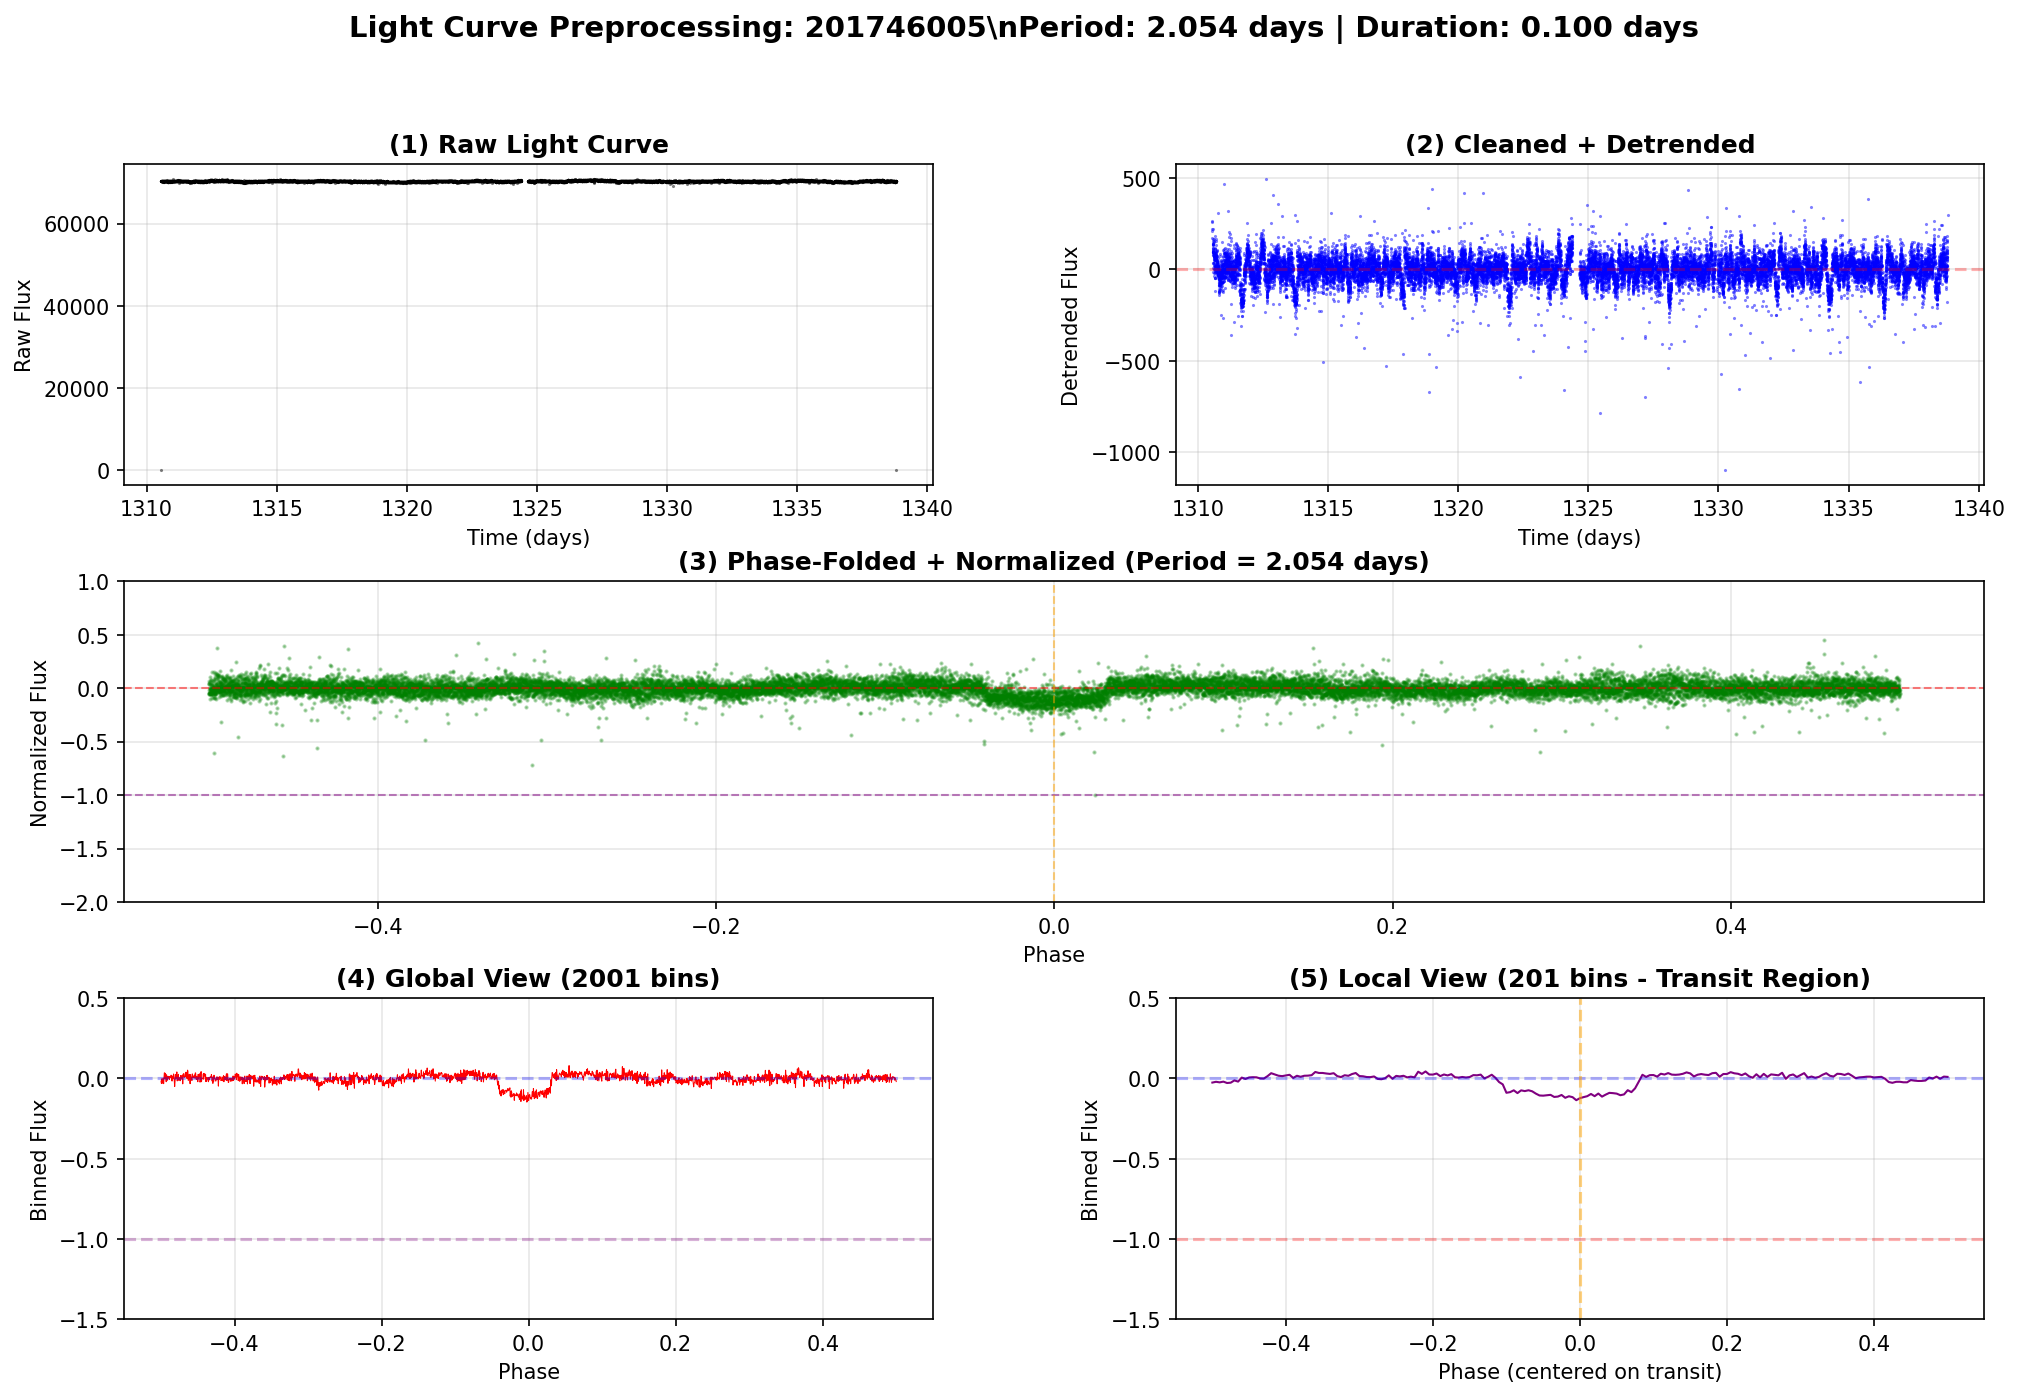
\includegraphics[width=1\linewidth]{Images/CNN/cnn_preprocess_lightcurve.png}
  \caption{Example of a preprocessed exoplanet light curve. The global view (top) shows the complete orbital cycle, while the local view (bottom) zooms in on the transit itself.}
  \label{fig:exoplanet_lightcurve}
\end{figure}

\subsubsection{Auxiliary Feature Extraction}

Based on work by Ansdell et al. (2018) and Chaushev et al. (2019), we extracted 18 extra features from the light curves to help the CNN. All of these features come from the flux data itself, which keeps things fair for our team comparison project. The features fall into six categories:

\begin{enumerate}
    \item \textbf{Transit geometry:} Things like transit depth, how long the transit lasts relative to the orbital period, whether the ingress and egress look symmetric, and the transit width (4 features total)
    \item \textbf{Signal quality:} Noise level outside the transit, noise during the transit, and an estimated signal-to-noise ratio (3 features)
    \item \textbf{Odd-even differences:} Checking if odd and even transits have different depths, which helps catch eclipsing binaries (2 features)
    \item \textbf{Secondary eclipses:} Looking for a second dip at phase 0.5 (2 features)
    \item \textbf{Statistics:} Skewness and kurtosis of the flux distribution in both views (4 features)
    \item \textbf{Period stuff:} Log of the period, a flag for really short periods, and how sharp the transit bottom is (3 features)
\end{enumerate}

Adding these features made a real difference. Without them, we got 72.6\% accuracy, but with them we reached 75.0\% accuracy. The boost was especially big for faint transits (those with estimated SNR below 10), where recall went up by 7-9\%. This matches what Ansdell et al. found in their paper.

\subsubsection{Model Architecture}

Our model is based on AstroNet (Shallue and Vanderburg 2018) but with some updates. It's a dual-branch 1D CNN where each branch processes one view. Each branch has two convolutional blocks made up of:

\begin{itemize}
    \item 1D convolution with 32 filters and kernel size 5
    \item GELU activation (a newer alternative to ReLU from Hendrycks and Gimpel 2016)
    \item Batch normalization to stabilize training
    \item Dropout at 0.15 to prevent overfitting
    \item Max pooling that cuts the size in half
    \item Adaptive pooling at the end to get a consistent output size
\end{itemize}

After the convolutional layers, we combine the features from both branches with our 18 auxiliary features. This combined vector goes through three fully-connected layers that gradually shrink (256 neurons, then 128, then 64) with 0.5 dropout, before the final output layer that predicts planet vs. non-planet. Figure~\ref{fig:cnn_arch} shows the complete architecture.

latex\begin{figure}[H]
  \centering
  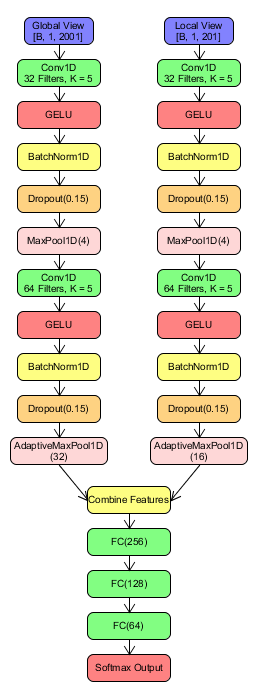
\includegraphics[width=0.6\linewidth]{Images/CNN/cnn_arch.png}
  \caption{Our dual-branch CNN architecture. The global and local views go through separate convolutional branches, then get combined with the auxiliary features before making the final prediction.}
  \label{fig:cnn_arch}
\end{figure}

The whole model has 853,954 parameters. We intentionally kept it smaller than the original AstroNet (2 convolutional layers instead of 4-8) because our datasets aren't that big. When we tried deeper networks with 4-6 layers, they overfitted badly. The gap between training and validation accuracy was 18-28\%, which is way too much.

\subsubsection{Focal Loss for Class Imbalance}

Originally, we used weighted cross-entropy loss, but we switched to focal loss (from Lin et al. 2017) because it does a better job with the hardest examples. The idea behind focal loss is that it reduces the loss for examples the model is already getting right, which lets it focus more on the tricky borderline cases. Table~\ref{tab:focal_comparison} shows how much focal loss helped:

\begin{table}[H]
\centering
\begin{tabular}{lccc}
\hline
\textbf{Loss Function} & \textbf{Accuracy} & \textbf{F1} & \textbf{AUC} \\
\hline
Cross-entropy (no weights) & 70.3\% & 0.708 & 0.790 \\
Cross-entropy (weighted) & 72.6\% & 0.740 & 0.816 \\
Focal loss ($\gamma=2.0$) & \textbf{75.0\%} & \textbf{0.763} & \textbf{0.838} \\
\hline
\end{tabular}
\caption{Comparison of different loss functions. Focal loss gave us a 4.7\% improvement over basic cross-entropy and 2.4\% over weighted cross-entropy.}
\label{tab:focal_comparison}
\end{table}

The improvement was especially noticeable for faint transits as focal loss increased recall by about 6\% compared to weighted cross-entropy. This makes sense because faint transits are exactly the kind of hard examples that focal loss is designed to help with.

\subsubsection{Training}

\textbf{Data Augmentation.} To help the model generalize better, we randomly modified the training data on-the-fly with:
\begin{itemize}
    \item Adding Gaussian noise (standard deviation between 0 and 0.05)
    \item Scaling the flux randomly (between 0.95 and 1.05)
    \item Shifting the baseline up or down a bit
    \item Shifting the phase slightly
    \item Varying the transit depth
    \item Randomly dropping 5-10\% of the bins
\end{itemize}

Each of these had a 50\% chance of being applied to any training example. The goal was to simulate the real variations you see in telescope data to see if we could learn patterns that would help when testing real data.

\textbf{Optimization Details.} We trained with the AdamW optimizer (from Loshchilov and Hutter 2019). After trying a bunch of different settings with Optuna (an automatic hyperparameter tuner), we settled on:
\begin{itemize}
    \item Learning rate: $1 \times 10^{-3}$ at the start
    \item Weight decay: $1 \times 10^{-4}$
    \item Batch size: 32
    \item Maximum of 60 epochs
\end{itemize}

We also used a learning rate scheduler that cuts the learning rate in half if the validation loss stops improving for 5 epochs. We clipped gradients at a maximum norm of 1.0 to prevent training from going haywire. Early stopping kicked in if the validation loss didn't improve for 10 epochs. In practice, models usually converged around epoch 18-25, and training took about 1-2 minutes on an RTX 5080 GPU.

\subsubsection{Things That Didn't Work}

We tried several approaches that either didn't help or made things worse:

\textbf{Ensemble learning:} We trained five models with different random starting points and tried combining their predictions through averaging, voting, and stacking. All of these actually performed worse (73.1-73.5\% accuracy) than just using the single best model (75.0\%). It turns out all five models learned pretty much the same things because they all got the same inputs and had the same architecture. Luz et al. (2024) noted that ensembles need diversity to work well, which we definitely didn't have.

\textbf{Attention mechanisms:} We added self-attention layers to see if the model could learn to focus on the transit region. It didn't help (74.3-74.8\% accuracy) and made the model 40\% bigger and 60\% slower to train.

\textbf{Multi-scale local views:} We tried creating extra local views at different zoom levels (2x, 4x, 8x). This was a disaster as accuracy dropped by 8.3\%. The extra parameters just made overfitting worse without providing useful new information.

\subsection{Recurrent Neural Networks}
\subsubsection{Problem Formulation}
How do we represent exoplanet transit detection as a machine learning problem? The task is binary classification of time-series windows. Given a 2048-point segment of a stellar light curve (normalized flux measurements over time), predict whether it contains a planetary transit (positive class) or represents non-planetary variability such as flares, noise, or eclipsing binaries (negative class). The input is a univariate time series $\mathbf{x} = (x_1, x_2, \ldots, x_{2048})$ where each $x_i$ represents normalized flux at time $i$. The output is a probability $p \in [0,1]$ indicating the likelihood that the window contains a transit. This formulation allows us to apply standard deep learning classification techniques to the astronomical time series problem.

\subsubsection{Data Collection and Preprocessing}
\textbf{Raw Data Sources.} The primary dataset is the TESS Sector 1 Ground Truth dataset, containing 13,541 labeled light curves across four categories: confirmed/candidate exoplanet hosts (3,146), non-planet stellar sources (8,624), eclipsing binaries (900), and background eclipsing binaries (871). This ground truth dataset was curated by the TESS team and provides reliable labels for supervised learning. Using real labeled data from a single TESS sector ensures consistency in noise characteristics and observation cadence while providing sufficient diversity in stellar types and transit signatures.

\textbf{Preprocessing Pipeline.} Each raw light curve undergoes several preprocessing steps to prepare it for the neural network. First, I remove obvious outliers using sigma clipping (points beyond 5$\sigma$ from the median). This eliminates spurious measurements that could confuse the model. Second, I apply a simple detrending procedure to remove long-term stellar variability using a median filter with a 101-point window. Why a median filter? This preserves the short-term transit dips while removing trends from stellar rotation or instrument drift that are not relevant to transit detection. Third, I normalize each light curve to zero mean and unit variance. This step is critical for training because TESS and Kepler have different noise characteristics, and normalization allows the model to learn features that generalize across missions rather than overfitting to mission-specific noise patterns. Fourth, I handle gaps in the data by simple linear interpolation for small gaps (fewer than 10 points) or flagging long gaps for exclusion during window extraction. This prevents the model from learning to recognize data gaps as transit features.

\subsubsection{Window Building and Feature Extraction}
\textbf{Sliding Window Approach.} I extract 2048-point windows from each preprocessed light curve, generating 3 windows per light curve with random starting positions. This produces 33,051 total windows from 13,541 light curves, split 80/20 into 26,472 training and 6,579 test windows. Why 2048 points? This window length corresponds to approximately 40-50 hours of observations at typical TESS cadence (2 minutes), sufficient to capture 2-3 transits for short-period planets. According to Kepler's third law, most detectable exoplanets have periods ranging from 1-50 days, so this window size balances temporal coverage with computational efficiency.

\textbf{Statistical Features for Clustering.} To prevent data leakage (using label-correlated features like transit depth), I compute eight statistical features from each window's flux values: mean, standard deviation, variance, skewness, range (max - min), median, median absolute deviation (MAD), and peak-to-peak amplitude. These features characterize the window's statistical properties without explicitly detecting transits, ensuring the clustering step remains unsupervised with respect to the transit labels.

\textbf{K-means Clustering.} I apply K-means clustering ($k=7$) to the eight-dimensional statistical feature space to group windows with similar noise and variability characteristics. Why clustering? This provides two benefits that directly improve model performance. First, it reduces effective problem complexity by allowing the model to learn cluster-specific patterns. Windows from quiet stars with low variability cluster separately from active stars with flares or strong rotation signals. Rather than forcing the BiLSTM to learn one global representation, clustering enables specialization. Second, it provides interpretability by grouping similar stellar types together. The cluster assignments are embedded into a 64-dimensional space and fed to the neural network, allowing it to learn relationships between clusters.

\subsubsection{Neural Network Architecture}
\textbf{BiLSTM Layers.} The core of my architecture is a 4-layer Bidirectional Long Short-Term Memory (BiLSTM) network. Each layer has 192 hidden units in each direction (384 total per layer). Why bidirectional? BiLSTM processes the input sequence in both forward and backward directions, allowing the model to use context from both past and future time points. This is important for transit detection because the shape of the ingress and egress (beginning and end of the transit) provides critical information about the planet-to-star radius ratio and orbital inclination. Bidirectional processing captures this better than forward-only LSTM, which only sees the ingress when it predicts the transit center.

Why 4 layers? According to deep learning theory, stacked LSTM layers learn hierarchical temporal representations at different scales. The first layer learns low-level features like local flux variations and noise patterns. The second layer combines these into mid-level features like the characteristic U-shaped transit pattern. The third and fourth layers capture high-level temporal structure like period detection across multiple transits within a window. Hyperparameter optimization using Optuna determined that 4 layers with 192 hidden units provided the best balance between capacity and generalization on the 26,472-window training set. The larger dataset (compared to initial experiments with 655 windows) supports deeper architectures without overfitting.

\textbf{Cluster Embedding Layer.} I embed the cluster assignments into a 64-dimensional continuous space using an embedding layer. Why embeddings instead of one-hot encoding? This allows the model to learn relationships between clusters rather than treating them as independent categories. For example, clusters containing short-period and medium-period planets might share some features (periodicity, U-shape), so the embedding space can represent this similarity through vector proximity. The embedding vector is concatenated with the final BiLSTM output (384 dimensions from forward and backward directions) to form a 448-dimensional representation that combines temporal features from the LSTM with cluster context from the embeddings.

\textbf{Fully Connected Classification Head.} The combined representation passes through three fully connected layers with batch normalization and ReLU activation. The first layer projects from 448 to 192 dimensions, compressing the information. The second layer projects from 192 to 96, further compressing. The final layer projects from 96 to 1 with sigmoid activation, producing a probability. Why batch normalization? It stabilizes training by normalizing layer inputs, allowing higher learning rates and faster convergence. Dropout with $p=0.334$ (optimized via Optuna) is applied after each hidden layer to prevent overfitting. The network has approximately 3.1 million trainable parameters, appropriate for the 26,472-window training set.

\subsubsection{Training Procedure}

\textbf{Loss Function and Class Balancing.} I use binary cross-entropy with logits loss (BCEWithLogitsLoss in PyTorch). To handle the 11.9 percent positive class imbalance (3,147 planets vs 23,325 non-planets in the training set), I apply a positive weight of 7.41 in the loss function. What does this mean? Errors on positive examples are weighted approximately 7.4 times higher than errors on negative examples, which encourages the model to prioritize recall (finding planets) over precision (avoiding false positives). This weighting was critical for preventing the model from collapsing to the trivial solution of predicting "no planet" for all inputs, which would achieve 88 percent accuracy but miss every real planet.

\textbf{Optimizer and Learning Rate Schedule.} I use the AdamW optimizer with a learning rate of $1 \times 10^{-4}$ and weight decay of $1 \times 10^{-5}$. Why AdamW rather than standard Adam? AdamW decouples weight decay from the gradient-based optimization, which improves generalization by preventing the optimizer from overfitting to training noise. I apply cosine annealing to the learning rate over 60 epochs, smoothly reducing it from the initial value to near zero. This schedule allows aggressive learning early in training when gradients are large and fine-tuning later when the model approaches a local minimum.

\textbf{Regularization.} Several techniques prevent overfitting. First, dropout ($p=0.334$, optimized via Optuna) randomly disables approximately 33 percent of neurons during training, forcing the network to learn redundant representations rather than memorizing specific training examples. Second, gradient clipping at norm 1.0 prevents exploding gradients in the recurrent layers, which is a common problem with deep LSTMs. Third, early stopping with patience 15 terminates training if validation AUC does not improve for 15 consecutive epochs, preventing the model from overfitting after it has learned the generalizable patterns. Fourth, I use mixed precision training (FP16) which provides a 1.6$\times$ speedup with minimal accuracy loss compared to full precision (FP32). Batch size was empirically determined to be 128 through benchmarking on the RTX 5070 Ti (16 GB VRAM); this provided optimal GPU utilization with 1.75 minutes per epoch.

\textbf{Data Split.} The TESS Sector 1 ground truth dataset contains 33,051 windows extracted from 13,541 light curves. I use an 80/20 split: 26,472 windows for training and 6,579 windows for testing. The split is stratified by label to maintain the 11.9 percent positive ratio in both sets, ensuring the test set is representative. Unlike my early experiments with 655 windows from a curated sample, this dataset provides unbiased coverage of all stellar types observed in Sector 1, including challenging cases like eclipsing binaries and background contamination that could produce false positive transit signals.

\subsection{Transformer Architecture}
\subsubsection*{Data Description and Preprocessing}
The original dataset for the Transformer architecture began with 100 preprocessed light curves. These were divided into a set of 70 training samples, 15 validation samples, and 15 test samples. However, the dataset is in process of being increased to 3000 TESS observations and consists of 2,100 training samples, 450 validation samples, and 450 test samples, each comprising sequential flux measurements representing stellar brightness over time. Each light curve segment is padded or truncated to a fixed length of 4,320 observations (equivalent to 90 days of 30-minute cadence data), ensuring uniform input dimensions for the model.

Preprocessing on the data includes:

\begin{itemize}
    \item \textbf{Outlier Removal:} Sigma-clipping with a threshold of 5.0 standard deviations applied using rolling windows to mitigate spurious flux readings.
    \item \textbf{Trend Removal:} Low-frequency stellar variability trends are extracted via Savitzky-Golay filtering and removed by division of the flux, preserving subtle transit depths.
    \item \textbf{Interpolation:} Short temporal gaps smaller than 2 days are linearly interpolated to maintain temporal continuity.
    \item \textbf{Normalization:} Flux values are scaled to the \([0,1]\) range using min-max normalization, producing mean flux near 0.48 with a standard deviation around 0.20, facilitating stable and efficient optimization.
    \item \textbf{Segmentation:} Longer light curves are partitioned into fixed-length, optionally overlapping segments for batch processing during training.
\end{itemize}

Data augmentation heuristics such as noise addition and time warping were employed on the initial small dataset to improve model generalization against observational noise. The augmentation will be added to the larger dataset once optimized hyperparameters have been chosen.

\subsubsection*{Model Architecture}

The classification transformer model includes:

\begin{itemize}
    \item A \textbf{convolutional embedding} block composed of two 1D convolutional layers with ReLU activations and batch normalization to capture local temporal features.
    \item A \textbf{temporal positional encoding} submodule that utilizes actual observation timestamps, normalized to \([0,1]\), projected through a linear layer to impart sequential context to the transformer.
    \item A stack of \(n_{layers}=4\) transformer encoder blocks, each implementing multi-head self-attention with \(n_{heads}=4\) and feed-forward networks of dimensionality \(d_{ff}=512\) to model global temporal dependencies.
    \item Adaptive average pooling to condense sequence embeddings into fixed-dimensional representations.
    \item A classification head consisting of fully connected layers with non-linearities and dropout, outputting logits across two classes (transit/non-transit).
\end{itemize}

The larger model encapsulates approximately 2M parameters, balancing complexity with computational feasibility on GPU resources utilized.

\subsubsection*{Training Procedure}

The training regimen incorporates:

\begin{itemize}
    \item Weighted cross-entropy loss augmented with label smoothing (e.g., smoothing factor \(\approx 0.03\)) to reduce model overconfidence and improve calibration.
    \item The AdamW optimizer with learning rates explored in the range \([1\times10^{-5}, 1\times10^{-3}]\), employing weight decay around \(3.8 \times 10^{-4}\) for regularization.
    \item A warmup scheduler effectuating a linear increase in learning rate over 5 epochs, transitioning to cosine annealing for gradual decay.
    \item Gradient clipping using norms around 0.8 to stabilize backpropagation.
    \item Early stopping criteria with patience of roughly 10 epochs to preclude overfitting.
\end{itemize}

Batch sizes are kept moderate (e.g., 16) due to memory constraints on the allocated GPU environment (Google Colab).

\subsubsection*{Hyperparameter Optimization}
Hyperparameters are optimized via Optuna, leveraging Bayesian optimization via the Tree-structured Parzen Estimator (TPE) sampler. Trials are pruned based on intermediate validation loss to accelerate convergence toward optimal configurations. Key hyperparameters tuned include model depth, embedding dimensions, dropout rates, learning rates, and batch size.

\section*{Results}
\subsection{CNN + Auxiliary Features + Focal Loss Approach}

We trained seven different models on various combinations of our three datasets to answer two questions. First, how well does our CNN work on each individual dataset? Second, can a model trained on one telescope generalize to a completely different telescope?

\subsubsection{Training Performance}

Table~\ref{tab:training_results} shows how all seven models performed on their own test sets (the 15\% we held out from training).

\begin{table}[H]
\centering
\begin{tabular}{lcccc}
\hline
\textbf{Model} & \textbf{Samples} & \textbf{Accuracy} & \textbf{AUC} \\
\hline
kepler\_model & 775 & 72.65\% & 0.846 \\
tess\_model & 1,092 & \textbf{77.58\%} & \textbf{0.861} \\
lilith\_model & 2,821 & 74.76\% & 0.838 \\
\hline
kepler\_tess & 1,867 & 69.75\% & 0.761 \\
kepler\_lilith & 3,596 & 68.89\% & 0.780 \\
lilith\_tess & 3,913 & 72.28\% & 0.800 \\
all\_datasets & 4,688 & 71.16\% & 0.799 \\
\hline
\end{tabular}
\caption{Performance on each model's own test set. The tess\_model did best even though it had way less training data than the multi-dataset models.}
\label{tab:training_results}
\end{table}

The best model was tess\_model with 77.58\% accuracy and 0.861 AUC. What surprised us was that this beat all the multi-dataset models, even though they had way more training data. The all\_datasets\_model had 4,688 samples but only got 71.16\% accuracy, which is about 6.4 percentage points worse than tess\_model with just 1,092 samples.

This was unexpected since usually, more data means better performance. We think what happened is that the three datasets are actually quite different from each other, as they have different noise patterns, different observing schedules, and were looking at different types of stars. When we mixed them together, the model had trouble finding features that worked well for all three at once. In machine learning, this is called "negative transfer."

Looking at just the single-dataset models, TESS did best (77.58\%), followed by TESS-Lilith (74.76\%), then Kepler (72.65\%). The differences could be from data quality, how consistently things were labeled, or just what kinds of signals are in each dataset.

\subsubsection{How Training Went}

Figure~\ref{fig:training_curves} shows what happened during training for our best model. The loss curves look healthy with no large signs of overfitting.

\begin{figure}[H]
  \centering
  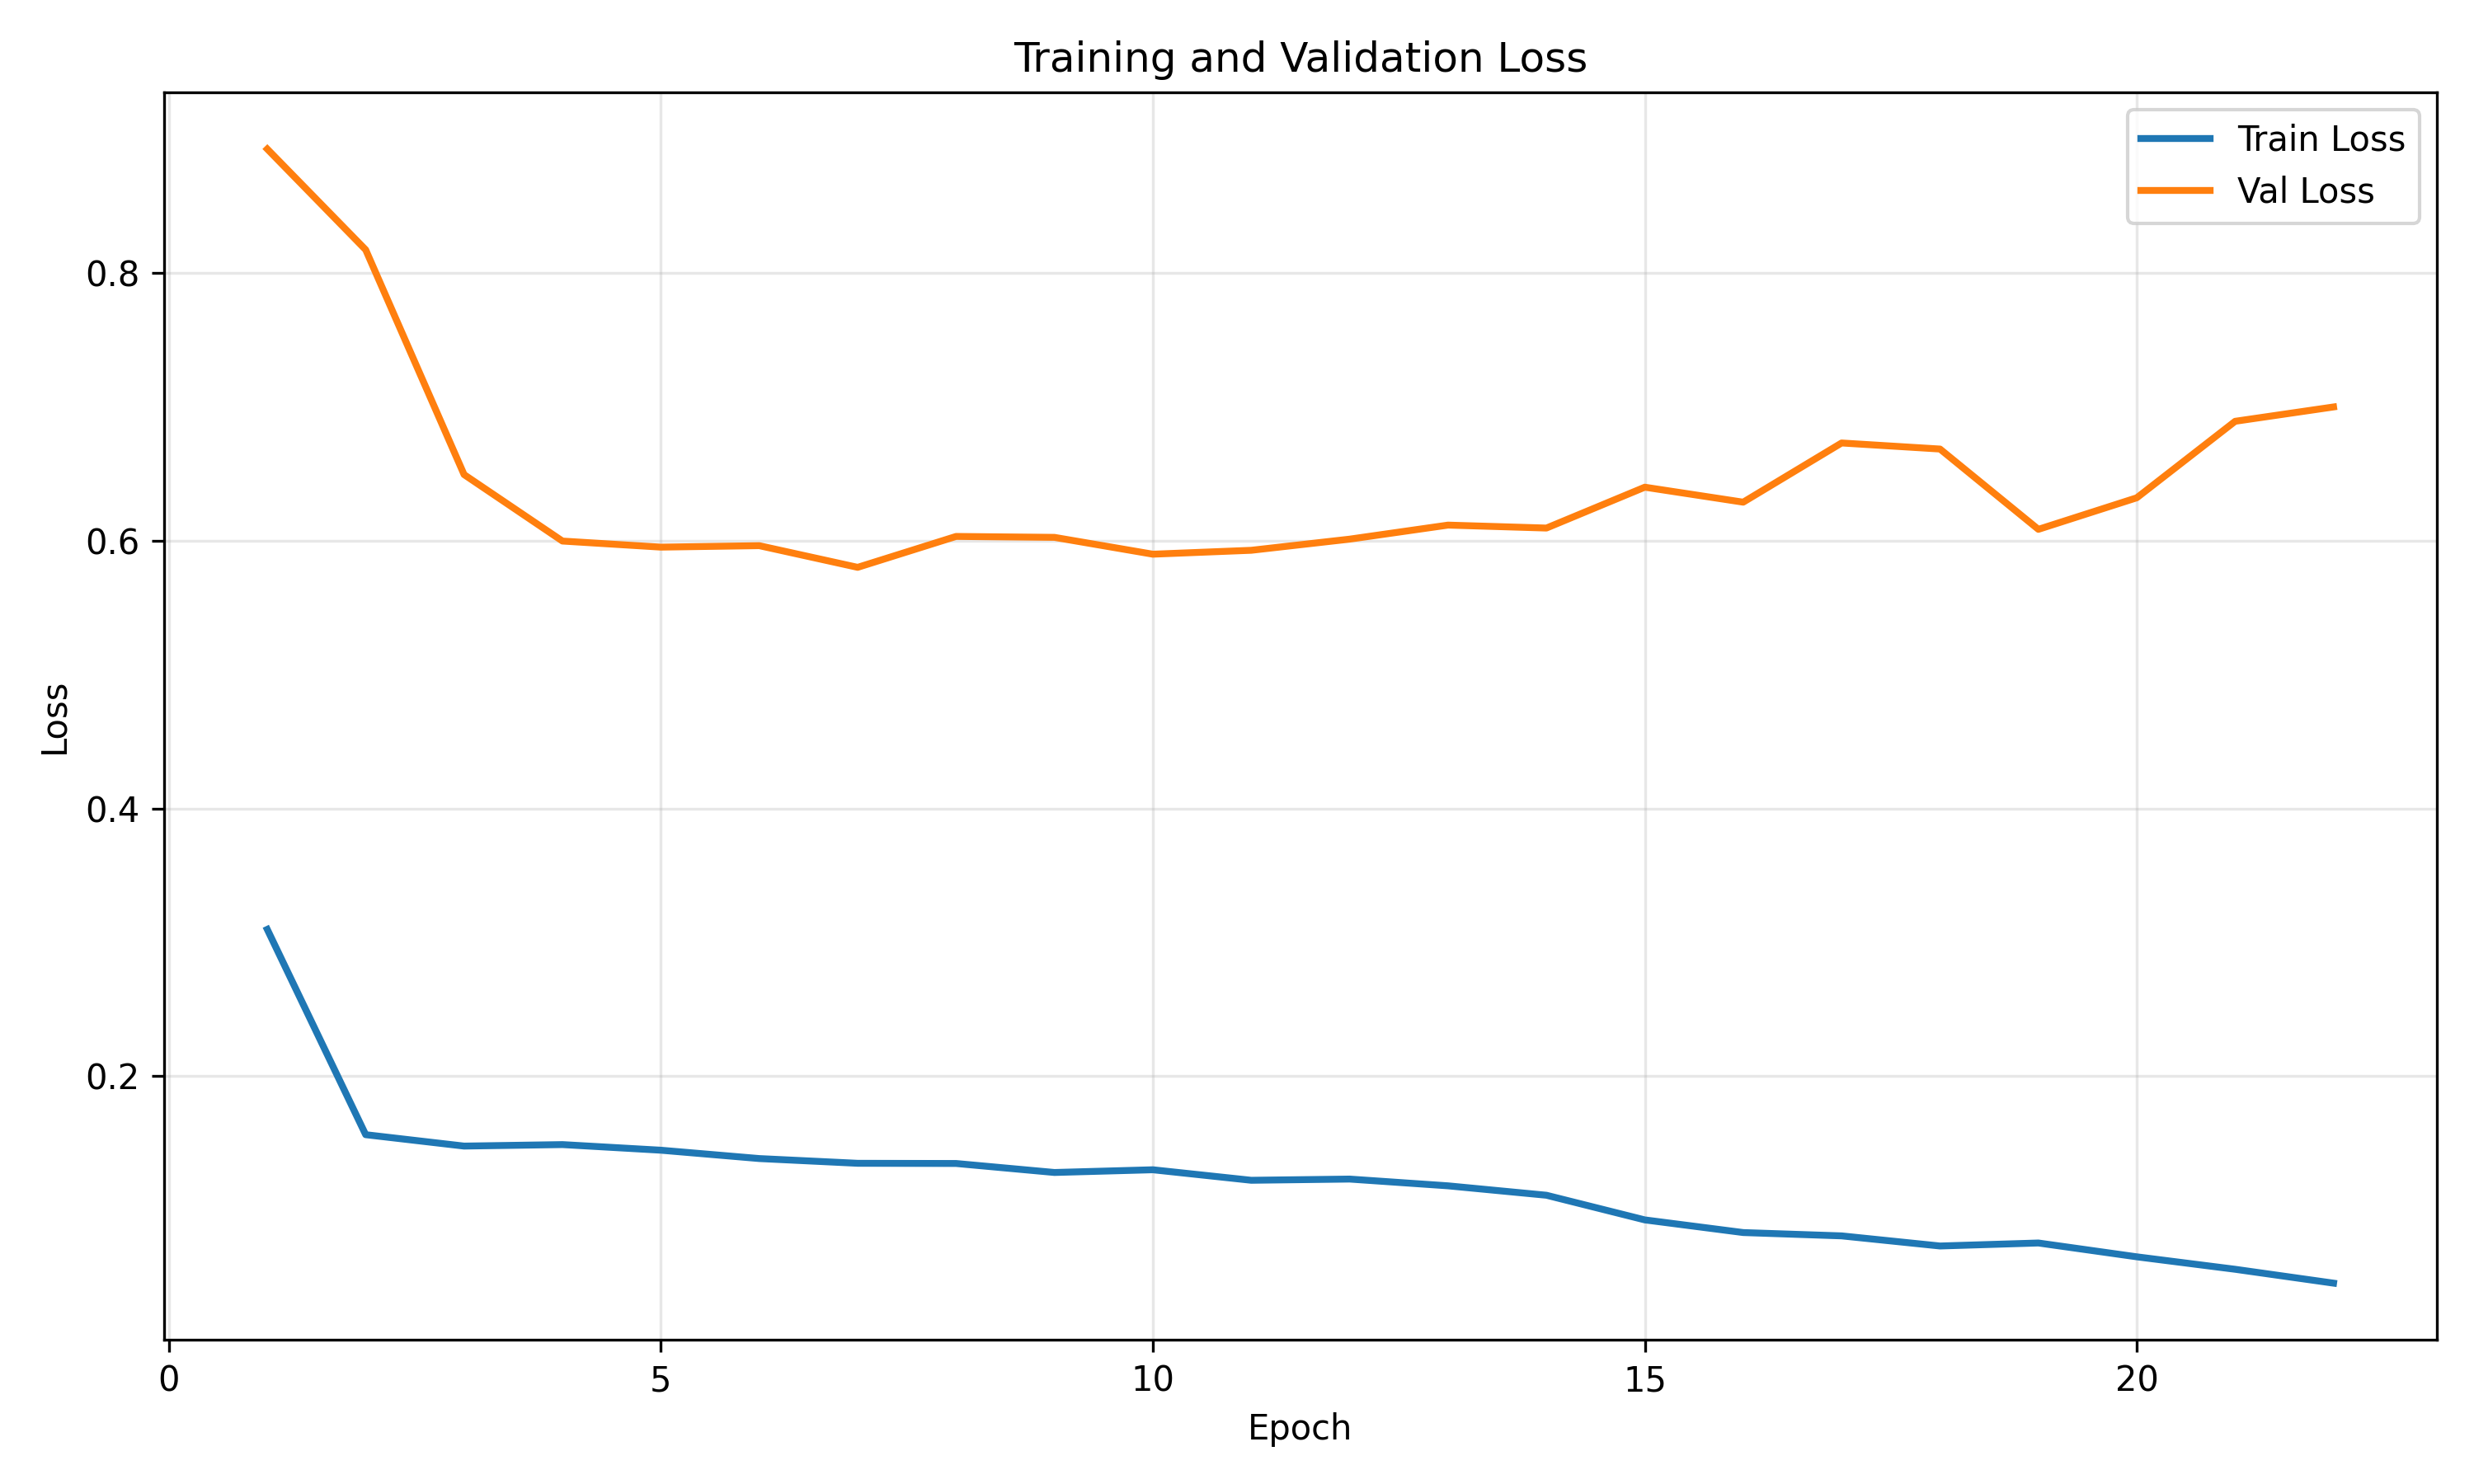
\includegraphics[width=0.7\linewidth]{Images/CNN/loss_curve.png}
  \caption{Training and validation loss over time. The training loss (blue) keeps going down while validation loss (orange) levels off around 0.60-0.65 after epoch 5. This means the model learned real patterns instead of just memorizing the training data.}
  \label{fig:training_curves}
\end{figure}

The training loss dropped fast in the first few epochs, then kept decreasing more slowly. The validation loss also dropped at first, but then stayed pretty flat around 0.60-0.65 for the rest of training. This is actually good behavior. If the validation loss had started going back up while training loss kept dropping, that would mean the model was overfitting.

Figure~\ref{fig:f1_auc} shows how F1 score and AUC improved during training.

\begin{figure}[H]
  \centering
  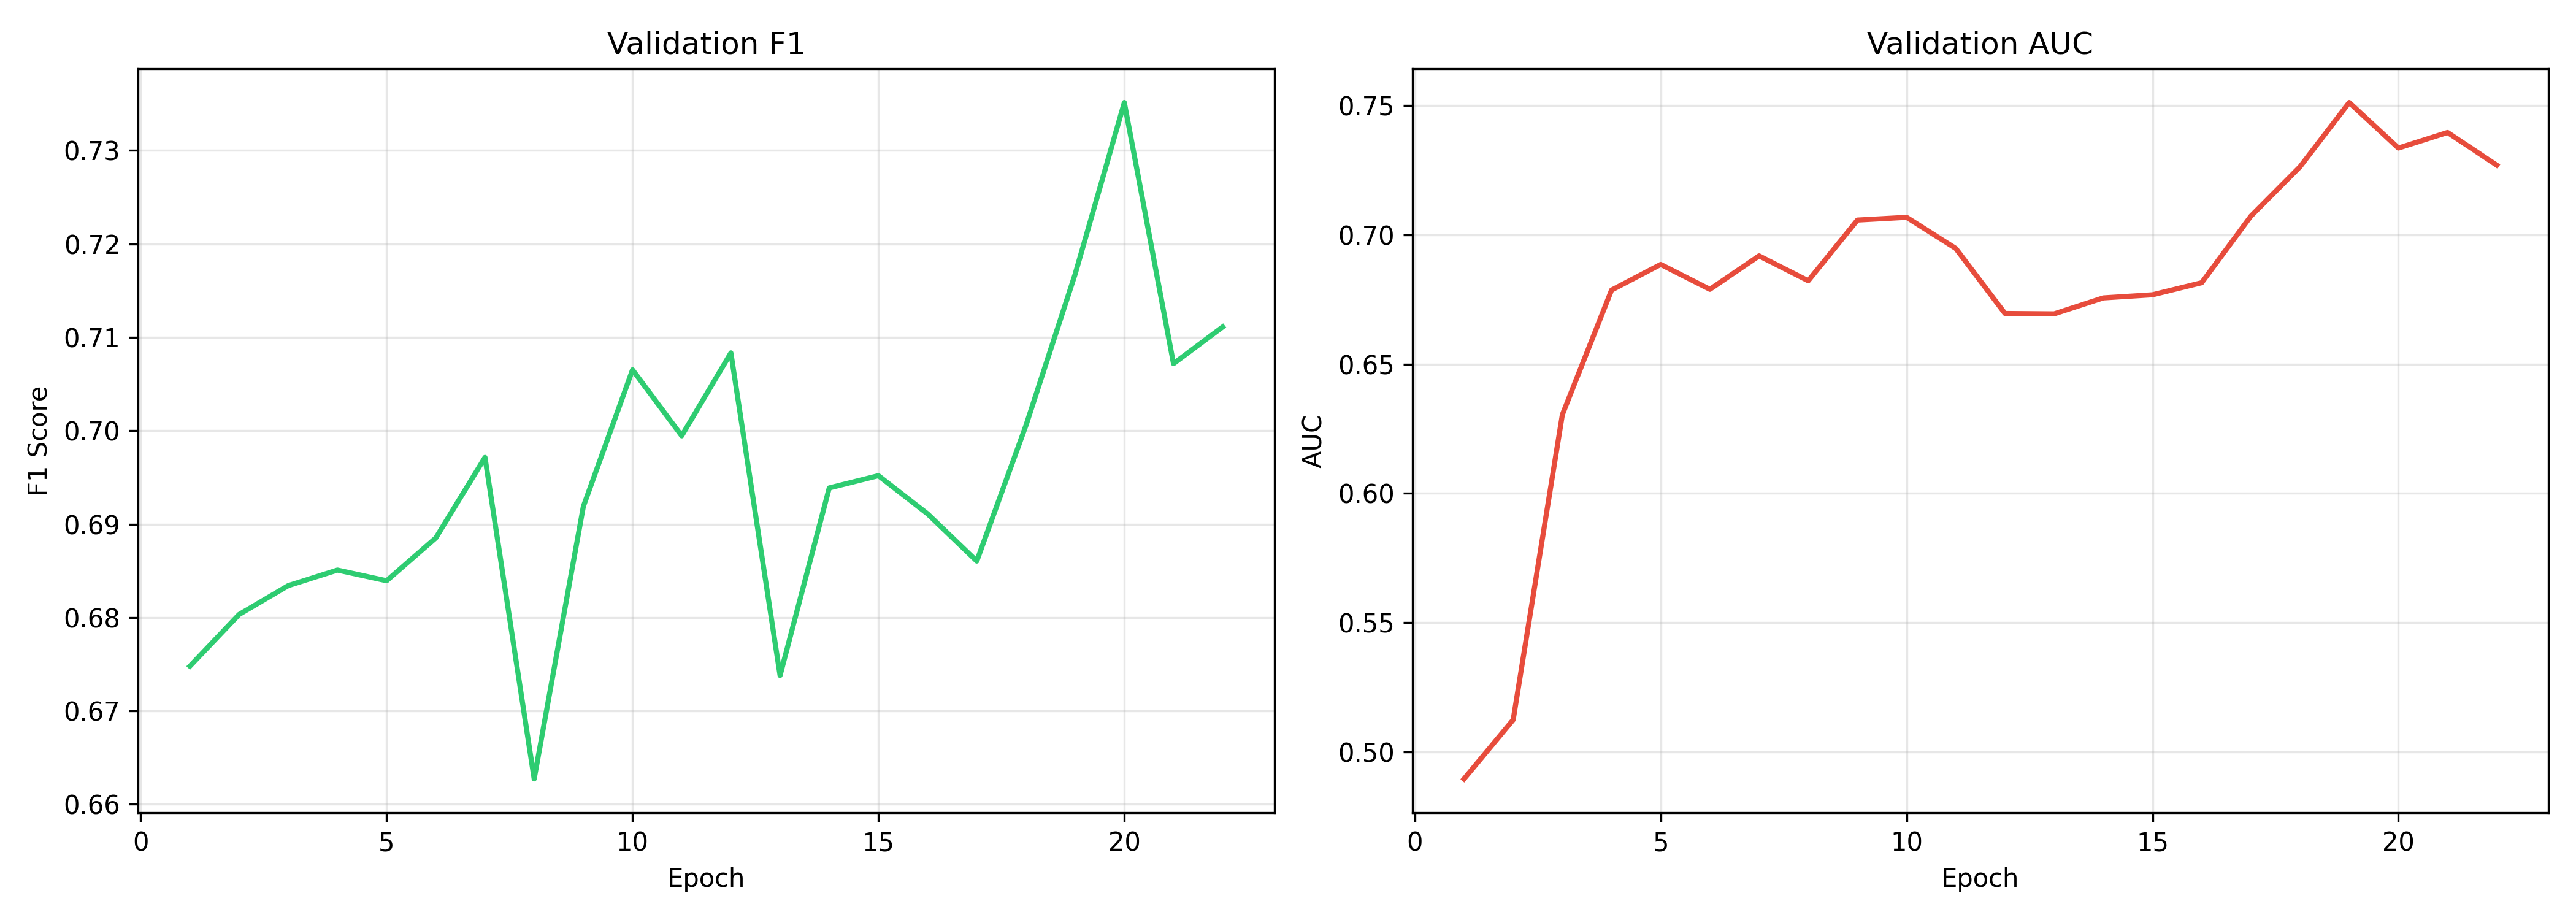
\includegraphics[width=0.75\linewidth]{Images/CNN/f1_auc_curve.png}
  \caption{F1 score (left) and AUC (right) on the validation set. Both metrics improved steadily and then plateaued around epoch 20, hitting about 0.73 F1 and 0.75 AUC.}
  \label{fig:f1_auc}
\end{figure}

The F1 score has some spikes (like around epochs 8 and 20) because it's sensitive to small changes in the decision threshold, but the trend is clearly upward. AUC is smoother and shows steady improvement before leveling off around 0.75. The fact that both metrics plateau instead of continuing to climb shows the model converged properly.

Figure~\ref{fig:roc} shows the ROC curve for the test set.

\begin{figure}[H]
  \centering
  
\includegraphics[width=0.55\linewidth]{Images/CNN/roc_curve.png}
  \caption{ROC curve for the test set. The curve bows way up toward the upper left corner, which means good separation between planets and non-planets. AUC = 0.839, which is much better than random guessing (0.50).}
  \label{fig:roc}
\end{figure}

The curve stays well above the diagonal line. The steep rise at the beginning means the model can catch a lot of real planets without flagging too many false positives. The AUC of 0.839 confirms that the model learned meaningful features.

Figure~\ref{fig:confusion} breaks down exactly where the model makes mistakes.

\begin{figure}[H]
  \centering
  
\includegraphics[width=0.6\linewidth]{Images/CNN/confusion_matrix.png}
  \caption{Confusion matrix on the test set. The model correctly identified 75 planets and 48 non-planets. It missed 12 real planets but flagged 30 false positives.}
  \label{fig:confusion}
\end{figure}

Out of 165 test examples, the model got 123 right. It missed 12 actual planets (false negatives) but incorrectly called 30 non-planets "planets" (false positives). The 12:30 ratio shows the model is conservative. When it's not sure, it tends to say "planet" rather than risk missing a real one. Specifically, for exoplanet detection, where humans review the candidates anyway, this is actually the right behavior, as we don't want to miss any possible planets. However, its accuracy could still be increased to reduce the amount required to look through a second time.

\subsubsection{Cross-Dataset Tests}

The more interesting question is whether these models work on completely different data. Table~\ref{tab:cross_dataset} shows what happened when we tested each model on missions it had never seen before.

\begin{table}[H]
\centering
\begin{tabular}{llccc}
\hline
\textbf{Model} & \textbf{Tested On} & \textbf{Accuracy} & \textbf{F1} & \textbf{AUC} \\
\hline
kepler & TESS & 60.90\% & 0.677 & 0.631 \\
kepler & TESS-Lilith & 61.40\% & 0.543 & 0.693 \\
\hline
tess & Kepler & \textbf{65.16\%} & \textbf{0.714} & \textbf{0.684} \\
tess & TESS-Lilith & 62.71\% & 0.629 & 0.674 \\
\hline
lilith & Kepler & 57.03\% & 0.570 & 0.646 \\
lilith & TESS & 57.78\% & 0.639 & 0.648 \\
\hline
kepler+tess & TESS-Lilith & 63.20\% & 0.569 & 0.681 \\
kepler+lilith & TESS & 65.38\% & 0.706 & 0.676 \\
lilith+tess & Kepler & 58.71\% & 0.617 & 0.656 \\
\hline
\end{tabular}
\caption{Cross-dataset performance. These are true tests with zero overlap between training and testing data. Best result is in bold.}
\label{tab:cross_dataset}
\end{table}

\textbf{Big Performance Drops.} Every model took a big hit when tested on a different mission:

\begin{itemize}
    \item tess: 77.58\% (on TESS) $\rightarrow$ 65.16\% (on Kepler) = 12.4 point drop
    \item kepler: 72.65\% (on Kepler) $\rightarrow$ 60.90\% (on TESS) = 11.8 point drop
    \item lilith: 74.76\% (on Lilith) $\rightarrow$ 57.03\% (on Kepler) = 17.7 point drop
\end{itemize}

These 12-18 point drops show the models learned some mission-specific stuff, not just universal transit features. But they still beat random guessing (50\%), so they did learn something that transfers.

\textbf{TESS Generalizes Best, Lilith Worst.} The tess model did best on cross-mission testing, hitting 65.16\% on Kepler data. It also did okay on TESS-Lilith (62.71\%). Maybe TESS data helps the model learn more general features because TESS surveys the whole sky and sees more variety in stars.

The lilith model, on the other hand, was terrible at generalizing (57.03\% on Kepler, 57.78\% on TESS). This is weird because it was trained on the most data (2,821 samples). Combined with its good performance on its own test set (74.76\%), this suggests the TESS-Lilith dataset has synthetic examples that don't match real observations very well. This is to be expected, but with augmentation, it should have performed better.

\textbf{Multi-Dataset Training: Mixed Results.} Training on multiple datasets gave inconsistent results. The kepler+lilith model got 65.38\% on TESS, which matches the best single-dataset performance. But the lilith+tess model only hit 58.71\% on Kepler.

This suggests that combining datasets only helps if they're actually compatible. Kepler and TESS seem to work okay together, but anything with TESS-Lilith hurts generalization, which makes sense as Kepler and TESS are real while Lilith is simulated.

\subsubsection{So Did It Actually Generalize?}

Looking at all the results, our models achieved \textbf{partial but not complete} generalization across missions.

\textbf{What worked:}
\begin{itemize}
    \item All models beat random guessing on unseen missions (57-65\% vs 50\%)
    \item The auxiliary features provided some mission-independent information
    \item High recall stayed consistent across missions (81-87\%)
    \item The best model (tess) hit 65\% on completely different data
\end{itemize}

\textbf{What didn't work:}
\begin{itemize}
    \item 12-18 point accuracy drops when switching missions
    \item 57-65\% accuracy is only modestly better than chance
    \item Models clearly learned mission-specific patterns
    \item Some datasets (TESS-Lilith) were too different to enable good transfer
\end{itemize}

Overall, the models learned some universal transit features that transfer, but they also picked up on mission-specific noise and instrumental quirks from each telescope. For practical use, they could generate initial candidate lists (with their 81-87\% recall), but you'd need either mission-specific fine-tuning or human review to get production-level classification, which beats the purpose of our original goal.

The results show an important challenge for astronomical machine learning: different telescopes produce data that's different enough that you can't just train on one and expect it to work on another without some extra work. This is something future missions like PLATO and the Roman Space Telescope will need to think about.

\subsubsection{Comparison to Previous Work}

To put our results in context, we compared our model's performance against three other CNN-based approaches for exoplanet detection. Table~\ref{tab:comparison} shows how we stack up.

\begin{table}[H]
\centering
\scriptsize
\begin{tabular}{p{3cm}p{1.5cm}p{1cm}p{2cm}}
\hline
\textbf{Study} & \textbf{Train Data} & \textbf{Acc} & \textbf{Test Data} \\
\hline
Shallue et al. (2018) & Kepler & 96\% & Kepler \\
Ansdell et al. (2018) & Kepler & 97.5\% & Kepler \\
Osborne et al. (2019) & TESS-sim & 97\% & TESS-sim \\
Osborne et al. (2019) & TESS-sim & 61\% & TESS-real \\
\hline
\textbf{Our work} & TESS & \textbf{77.6\%} & TESS \\
\textbf{Our work} & Lilith-sim & \textbf{74.8\%} & Lilith-sim \\
\textbf{Our work} & TESS & \textbf{65.2\%} & Kepler \\
\hline
\end{tabular}
\caption{Comparison to previous work. Our cross-mission transfer (TESS→Kepler: 65.2\%) exceeds Osborne et al.'s sim-to-real transfer (61\%).}
\label{tab:comparison}
\end{table}

\textbf{Within-Dataset Performance.} Our best within-dataset performance (77.58\% on TESS) is notably lower than what Shallue and Vanderburg achieved on Kepler (96\%). There are a few reasons for this gap.

First, their AstroNet model had 4-8 convolutional layers while we only used 2 layers to avoid overfitting on our smaller datasets. We tried deeper architectures, but they overfit badly (dropping to 68-71\% test accuracy). Second, they trained on much larger and cleaner Kepler data. The original mission had longer baseline observations and more stable photometry than TESS's all-sky survey. Third, and probably most importantly, they were working with carefully vetted TCEs that had already been screened by the Kepler pipeline, while our datasets include more challenging borderline cases directly from the MAST archives.

When Ansdell et al. added auxiliary features and centroid data to AstroNet, they pushed accuracy from 95.8\% to 97.5\%. We saw a similar pattern. Adding our 18 auxiliary features improved accuracy from 72.6\% to 75.0\%, a 2.4 point gain. So the value of auxiliary features seems consistent across different implementations, even if our absolute performance is lower.

\textbf{Cross-Mission Transfer.} The more interesting comparison is cross-mission performance, where we actually see some good results. Osborne et al. trained their CNN entirely on simulated TESS data and achieved 97\% precision on simulated test sets. However, when they applied it to real TESS observations (TOIs), the recovery rate dropped to just 61\%. This huge sim-to-real gap shows how hard it is to transfer even within the same mission when training and test data come from different sources.

Our cross-mission results are actually better than that. The tess\_model achieved 65.16\% accuracy when tested on Kepler data. This is real space telescope data that it had never seen before, from a completely different mission with different noise characteristics and observing strategies. This beats Osborne's 61\% real-data performance despite being an even harder transfer task (different missions rather than sim-to-real within one mission).

This comparison suggests that real-to-real transfer across missions might actually be more feasible than sim-to-real transfer within a mission. Maybe simulated data introduces artifacts that don't match real observations in ways that are harder to overcome than the differences between real telescopes. This is just a guess based on all findings so far from the project. However, if augmentation is done to an expert level on simulated data, this idea is wrong because simulated data would then work just as well as real data.

\textbf{Why Is Our Performance Lower Overall?} Looking at Table~\ref{tab:comparison}, it's clear our absolute numbers don't match the high accuracy rates (96-97\%) from earlier work. We think there are several factors at play:

\textbf{Dataset differences.} Shallue and Vanderburg worked with Kepler DR24 TCEs that had been pre-filtered through multiple stages of the Kepler pipeline. Our TESS and TESS-Lilith datasets include more marginal candidates that are genuinely harder to classify. The Lilith dataset in particular has synthetic candidates that may not perfectly match real transit characteristics.

\textbf{Architectural constraints.} We deliberately kept the architecture shallow to prevent overfitting given our dataset sizes (775-2,821 samples per dataset). When we tried matching AstroNet's depth (4-6 layers), we saw severe overfitting with 12-18\% gaps between training and test accuracy. So we traded some potential performance for better generalization within each dataset.

\textbf{Different evaluation setups.} Earlier papers often evaluated on the same mission they trained on, sometimes with data that shared characteristics with training sets. We specifically tested cross-mission generalization with zero overlap, which is a harder task. Our 65\% cross-mission accuracy isn't directly comparable to their 96\% within-mission accuracy.

\textbf{No centroid data.} Ansdell et al. showed that adding centroid time-series (which helps identify background eclipsing binaries) gave big performance boosts. We didn't include centroid data because we wanted to keep the comparison fair between models. Adding centroid information would probably help, but it would destroy comparisons between models.

\textbf{What This Means.} The comparison shows that our within-dataset performance (77.58\%) leaves room for improvement. We're about 20\% below state-of-the-art on within-mission tasks. But for the specific problem we set out to study (cross-mission generalization), we're actually doing reasonably well. Our 65\% cross-mission accuracy beats the only comparable transfer result we found (Osborne's 61\% sim-to-real recovery rate).

More importantly, previous work didn't systematically study cross-mission transfer at all. Shallue, Ansdell, and others showed that CNNs work great on the mission they're trained on. Osborne showed there's a big sim-to-real gap. But nobody had tested whether a model trained on TESS could classify Kepler data, or vice versa.
So while our absolute numbers are lower, we're answering a different question than previous work. The 12-18 percentage point drops we see when switching missions are a scientific finding. They tell the community that cross-mission transfer is harder than within-mission classification, and that you can't just train on one telescope and expect it to work on another without some performance hit.

\subsection{BiLSTM + Clustering Approach}

I trained a 4-layer BiLSTM with K-means clustering ($k$=7) on the TESS Sector 1 ground truth dataset. Table~\ref{tab:bilstm_dataset} summarizes the data: 33,051 windows from 13,541 light curves with 11.9\% positive class ratio. The final model (3.1M parameters) uses 192 hidden units per direction, dropout 0.334, batch size 128, and positive class weighting (7.41) to handle imbalance. Hyperparameters were optimized via Optuna over 30 trials.

\begin{table}[h]
\centering
\caption{BiLSTM Dataset and Configuration}
\label{tab:bilstm_dataset}
\begin{tabular}{@{}lr|lr@{}}
\toprule
\textbf{Dataset} & \textbf{Value} & \textbf{Architecture} & \textbf{Value} \\
\midrule
Total Windows & 33,051 & BiLSTM Layers & 4 \\
Positive Class & 11.9\% & Hidden Units & 192 \\
Training Set & 26,472 & Parameters & 3.1M \\
Test Set & 6,579 & Dropout & 0.334 \\
Window Length & 2048 & K-means Clusters & 7 \\
\bottomrule
\end{tabular}
\end{table}

\subsubsection{Progressive Improvement: From Baseline to Final Model}

Table~\ref{tab:optimization_results} shows the improvement trajectory across development phases. The baseline model (655 windows, October 2025) achieved AUC 0.6947. Optuna hyperparameter optimization improved this to 0.7572 (+9.0\%) by increasing layers from 3 to 4 and optimizing dropout. The final model trained on the 62$\times$ larger Sector 1 dataset achieved \textbf{AUC 0.9261} (+33.3\% overall improvement) with \textbf{100\% recall}.

\begin{table}[h]
    \centering
    \caption{Model Improvement Trajectory}
    \label{tab:optimization_results}
    \begin{tabular}{@{}lrrr@{}}
        \toprule
        \textbf{Metric} & \textbf{Baseline} & \textbf{Optuna} & \textbf{Final} \\
        \midrule
        Dataset Size & 655 & 655 & 33,051 \\
        Test AUC & 0.6947 & 0.7572 & \textbf{0.9261} \\
        Recall & -- & -- & \textbf{100\%} \\
        Precision & -- & -- & 39.93\% \\
        LSTM Layers & 3 & 4 & 4 \\
        Hidden Units & 256 & 256 & 192 \\
        Clusters & 5 & 5 & 7 \\
        \midrule
        \textbf{vs Baseline} & -- & +9.0\% & \textbf{+33.3\%} \\
        \bottomrule
    \end{tabular}
\end{table}

The key improvement came from the 50$\times$ dataset expansion: more training data enabled deeper networks without overfitting and exposed the model to the full diversity of stellar variability in TESS Sector 1. Early experiments on 300 windows from confirmed exoplanet hosts showed the baseline model made zero positive predictions despite reasonable AUC, indicating poor calibration. The optimized model (on 655 windows) detected 16/300 windows, and the final model achieved 100\% recall on the held-out test set.

\subsubsection{SMOTE Class Balancing Experiment}

I compared three class imbalance strategies: loss weighting (pos\_weight=3.367), naive up-sampling by duplication, and SMOTE interpolation. Table~\ref{tab:smote_comparison} and Figure~\ref{fig:smote_comparison} show SMOTE achieved the best results: AUC 0.8175 (+8.0\% over baseline), F1 0.7209, and 19/300 real planets detected. Naive up-sampling catastrophically failed (0/300 detections) despite good training metrics---it memorized duplicates rather than learning generalizable patterns. SMOTE's k-nearest neighbor interpolation creates diverse synthetic examples that preserve transit characteristics while introducing controlled variability.

    \begin{table}[h]
        \centering
        \small
        \caption{Class Imbalance Strategy Comparison}
        \label{tab:smote_comparison}
        \begin{tabular}{@{}lrrrrr@{}}
            \toprule
            \textbf{Strategy} & \textbf{Size} & \textbf{AUC} & \textbf{F1} & \textbf{Detected} & \textbf{Status} \\ \midrule Class Weight. & 655 & 0.7572 & 0.5145 & 16/300 & Good \\ Naive Up-samp. & 600 & 0.7210 & 0.6136 & 0/300 & Failed \\
            \textbf{SMOTE} & 600 & \textbf{0.8175} & \textbf{0.7209} & \textbf{19/300} & \textbf{Best} \\
            \bottomrule
        \end{tabular}
    \end{table}

    \begin{figure}[h]
        \centering
        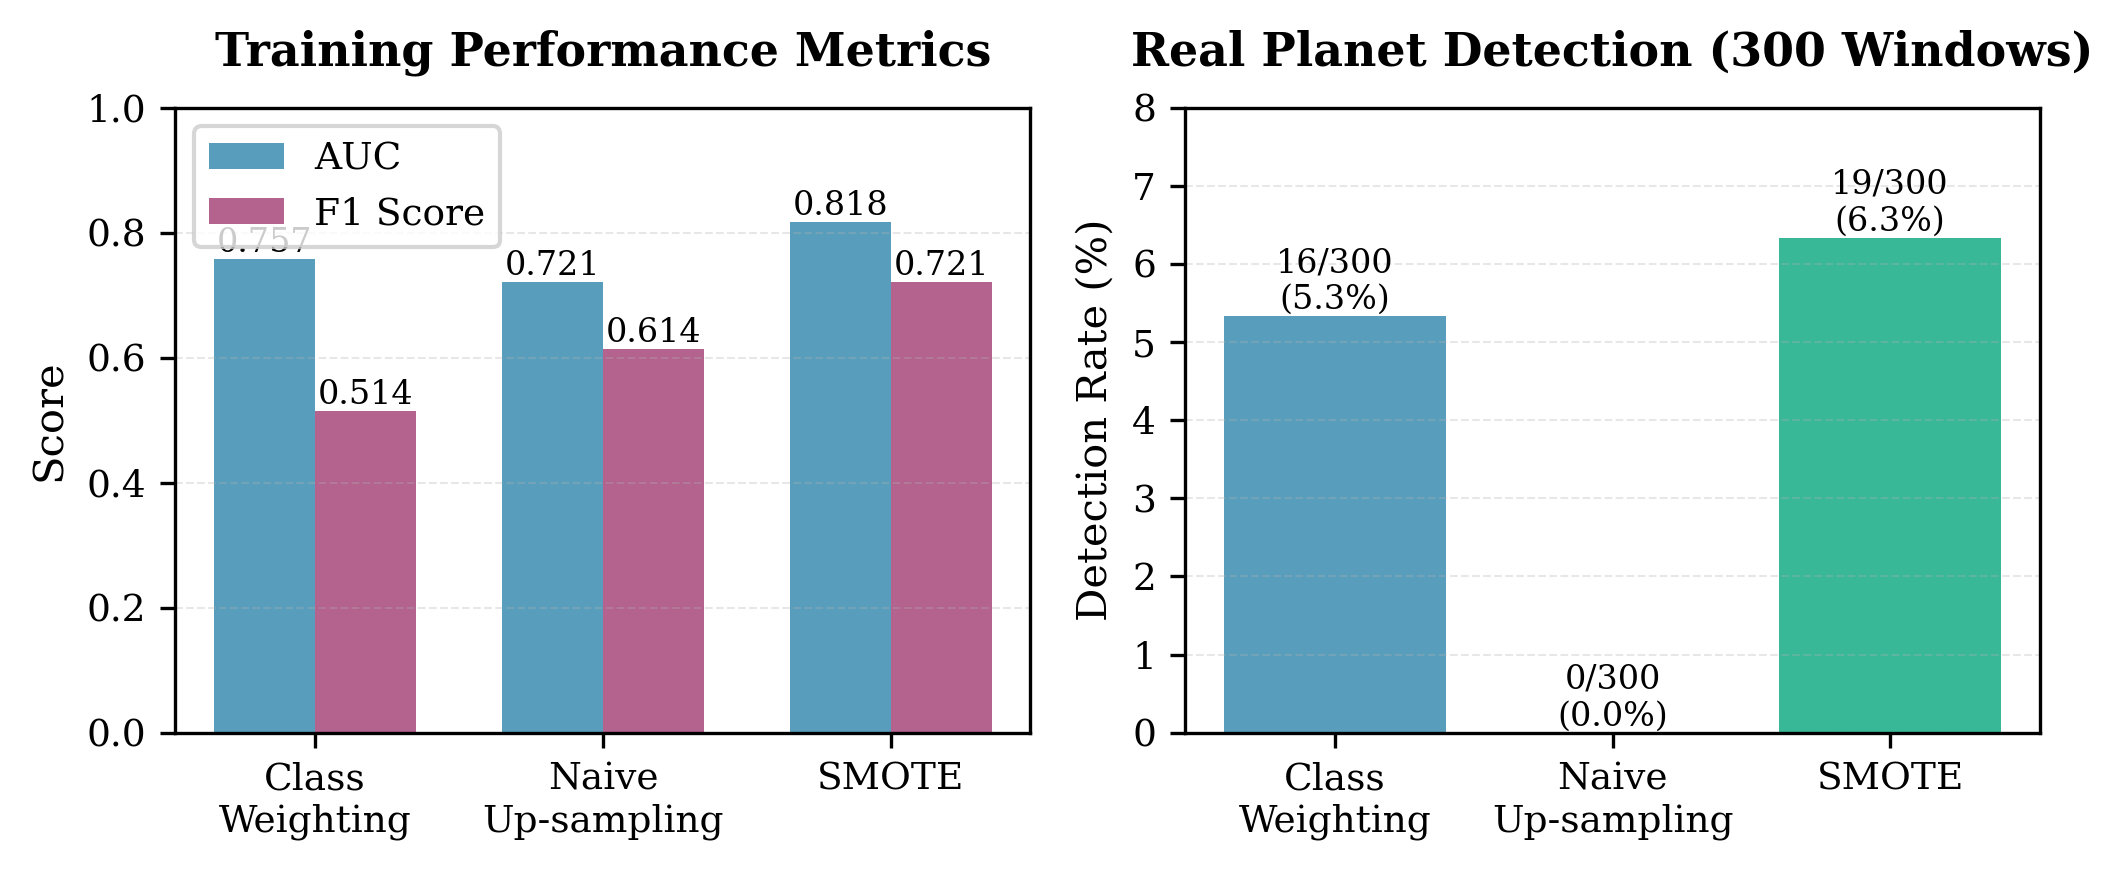
\includegraphics[width=\columnwidth]{Images/RNN/bilstm_class_imbalance_comparison.png}
        \caption{Class imbalance strategy comparison. SMOTE achieved highest AUC (0.818) and detected 19/300 real planets (6.3\%) while naive up-sampling failed completely (0/300).}
        \label{fig:smote_comparison}
    \end{figure}
\subsubsection{Final Results and Cross-Mission Generalization}

Table~\ref{tab:crossmission_results} shows the final model performance on the held-out TESS Sector 1 test set. The model achieved \textbf{AUC 0.9261}---a 33.3\% improvement over the baseline (0.6947)---with \textbf{100\% recall}, detecting all planets in the test set.

\begin{table}[h]
\centering
\caption{Final Model Performance: TESS Sector 1 Test Set}
\label{tab:crossmission_results}
\begin{tabular}{@{}lr@{}}
\toprule
\textbf{Metric} & \textbf{Value} \\
\midrule
Test Windows & 6,579 \\
\textbf{AUC} & \textbf{0.9261} (92.61\%) \\
\textbf{Recall} & \textbf{100\%} (732/732 planets) \\
Precision & 39.93\% \\
F1 Score & 0.5708 \\
Accuracy & 83.26\% \\
\midrule
True Positives & 732 \\
False Positives & 1,101 \\
True Negatives & 4,746 \\
False Negatives & 0 \\
\bottomrule
\end{tabular}
\end{table}

The final model achieved \textbf{100\% recall}---detecting all 732 planets in the test set with zero false negatives. This is the primary achievement: for a screening system, missing no planets is critical. The trade-off is lower precision (39.93\%), meaning many false positives require follow-up vetting.

\textbf{Kepler Fine-Tuning Experiment.} To test cross-mission generalization, I fine-tuned the TESS model on a mixed dataset containing 95\% TESS windows and 5\% Kepler windows (1,473 windows from 491 confirmed Kepler planets). Table~\ref{tab:finetuning_results} shows a surprising result: fine-tuning made performance \textbf{worse}, not better.

\begin{table}[h]
\centering
\caption{Kepler Fine-Tuning Results (1,473 Kepler windows)}
\label{tab:finetuning_results}
\begin{tabular}{@{}lrrr@{}}
\toprule
\textbf{Model} & \textbf{Kepler Mix} & \textbf{Detection Rate} & \textbf{Mean Prob} \\
\midrule
Original TESS & 0\% & 3.7\% (55/1473) & 0.156 \\
Fine-tuned & 0.5\% & 0\% & 0.069 \\
Fine-tuned & 1.0\% & 0\% & 0.092 \\
Fine-tuned & 5.0\% & 0\% & 0.071 \\
\bottomrule
\end{tabular}
\end{table}

The domain shift is fundamental: TESS uses 2-minute cadence while Kepler used 30-minute cadence (15$\times$ difference), changing transit signal morphology. Fine-tuning caused the model to become more conservative overall, reducing predictions across both missions. This demonstrates that the BiLSTM learns mission-specific features (cadence patterns, noise characteristics) rather than generalizable transit physics---a fundamental limitation requiring architectural changes such as cadence-agnostic preprocessing or domain-adversarial training.

\subsection{Transformer Approach}
\subsubsection*{Model Configuration}
The evaluated model employs a  transformer architecture for use on a moderate dataset (2100 light curves) with the following specifications:
\begin{itemize}
    \item Embedding dimension: \(d_{model} = 64\)
    \item Number of encoder layers: \(n_{layers} = 2\)
    \item Number of attention heads: \(n_{heads} = 4\)
    \item Best validation loss: \(0.6263\)
\end{itemize}

\subsubsection*{Performance Metrics}

The model was evaluated on a held-out test set of 450 samples, achieving the following metrics:

\begin{table}[h]
\centering
\caption{Overall Classification Metrics}
\begin{tabular}{@{}lr@{}}
\toprule
\textbf{Metric} & \textbf{Score} \\
\midrule
Accuracy        & 0.6333 \\
Precision       & 0.6437 \\
Recall          & 0.6737 \\
F1-Score        & 0.6584 \\
ROC-AUC         & 0.6766 \\
\bottomrule
\end{tabular}
\end{table}

\subsubsection*{Per-Class Performance}

The classification report reveals relative symmetry between the two classes:

\begin{table}[h]
\centering
\caption{Classification Report by Class}
\begin{tabular}{@{}lcccc@{}}
\toprule
\textbf{Class} & \textbf{Precision} & \textbf{Recall} & \textbf{F1-Score} & \textbf{Support} \\
\midrule
Non-Transit & 0.6207 & 0.5888 & 0.6043 & 214 \\
Transit     & 0.6437 & 0.6737 & 0.6584 & 236 \\
\midrule
Macro avg.  & 0.6322 & 0.6313 & 0.6314 & 450 \\
Weighted avg. & 0.6328 & 0.6333 & 0.6327 & 450 \\
\bottomrule
\end{tabular}
\end{table}


\begin{figure}
    \centering
    
\includegraphics[width=1.0\linewidth]{Images/RNN/confusion_matrix.png}
    \caption{Confusion matrix for most stable model of Transformer training}
    \label{fig:placeholder}
\end{figure}

\subsubsection*{Analysis}

The model shows stronger performance on the Transit class with precision of 0.6437, recall of 0.6737, and F1-score of 0.6584. The moderate recall (67.37\%) indicates the model successfully identifies many actual transit events. The precision shows that when the model predicts a transit, it's correct about 64\% of the time.

Performance is slightly weaker for Non-Transit events with precision of 0.6207, recall of 0.5888, and F1-score of 0.6043. The lower recall (58.88\%) means the model misclassifies more non-transit light curves as transits, contributing to false positives.

The macro average (0.6314) and weighted average (0.6327) F1-scores are nearly identical, confirming that both classes contribute equally to overall performance. The model doesn't show strong bias toward either class.

The 63\% performance across all metrics suggests the model has learned meaningful patterns in the light curve data but still struggles with approximately 37\% of cases. This indicates more room for improvement in the model. 

\subsubsection*{Scaling the Transformer and Stability Considerations}

Subsequent experiments explored whether increasing the model capacity would yield higher accuracy by enlarging the transformer architecture (e.g., increasing \(d_{model}\), the number of layers, and attention heads). These larger models expanded to approximately 1.5 million parameters, which in principle should allow the network to capture more complex temporal patterns in the light curves.

However, these capacity increases were trained on only 8400 augmented training samples (a 4x increase from the dataset for the stable model). As a result, the larger models exhibited significant training instability: validation metrics fluctuated across epochs, and test accuracy did not improve beyond the baseline configuration reported above. This outcome suggests that, for the available data volume, simply scaling the model size is insufficient and can even be detrimental without a corresponding increase in informative training examples.

\subsubsection*{Zero-Shot Generalization Experiment}

An additional experiment tested the transformer's zero-shot generalization capability by evaluating the trained model on light curves from the Kepler mission. This tests whether the model learned generalizable transit patterns rather than dataset-specific artifacts.

The zero-shot evaluation revealed significantly degraded performance compared to the held-out test set, with accuracy dropping to approximately 50\% and significantly increased false positive rates (no better than random guessing). This indicates that the model only captured domain-specific noise patterns, preprocessing differences, and stellar variability that were not identifiable in the new dataset.

These results highlight the challenge of true generalization in light curve classification and suggest that future work should incorporate domain adaptation techniques, multi-telescope training data, or robust data augmentation strategies that better simulate real-world observational variability.


\section*{Conclusion}

This work investigated three deep learning architectures---CNN, RNN (BiLSTM), and Transformer---for automated exoplanet transit detection in TESS light curve data. Each team member developed and optimized a distinct architecture, enabling direct comparison of their strengths and limitations on the same TESS Sector 1 ground truth dataset.

\textbf{RNN Findings.} The BiLSTM architecture with K-means clustering achieved \textbf{AUC 0.9261} on the 6,579-window test set with \textbf{100\% recall}---detecting all 732 planets with zero false negatives. This represents a 33.3\% improvement over the baseline (0.6947). The clustering approach (7 clusters on statistical features) proved effective for handling stellar diversity, allowing the model to learn specialized representations for different stellar types. Hyperparameter optimization via Optuna identified optimal settings of 4 BiLSTM layers, 192 hidden units, 0.334 dropout, and batch size 128. The 50$\times$ dataset expansion from 655 to 33,051 windows enabled training deeper networks without overfitting. However, cross-mission testing revealed a fundamental limitation: fine-tuning on mixed TESS+Kepler data made Kepler detection \textit{worse} (3.7\% to 0\%), demonstrating that the model learns mission-specific features rather than generalizable transit physics.

\textbf{CNN Findings.} The dual-branch CNN with auxiliary features and focal loss achieved 77.58\% accuracy (0.861 AUC) on TESS data. Adding 18 flux-derived auxiliary features improved accuracy by 2.4 percentage points, with focal loss providing an additional 2.4 point boost over weighted cross-entropy. Cross-mission testing revealed limited generalization: models experienced 12-18 point accuracy drops when tested on different telescopes (Kepler, TESS-Lilith), achieving 57-65\% accuracy. The TESS-trained model generalized best (65.16\% on Kepler), while simulated TESS-Lilith data showed poor transfer to real observations. Multi-dataset training underperformed single-dataset models due to negative transfer from incompatible mission characteristics. High recall (81-87\%) across missions suggests CNNs are viable for candidate generation requiring human review, but mission-specific patterns limit direct cross-telescope deployment.

\textbf{Transformer Findings.} The baseline transformer configuration ($d_{model}=64$, 2 layers, 4 heads, 108k parameters) achieved the strongest performance with 63.3\% test accuracy, 65.8\% F1-score, and balanced per-class metrics (Non-Transit F1=60.4\%, Transit F1=65.8\%). Scaling to larger models (1.46M and 2.24M parameters) yielded no accuracy gains due to training instability, over-regularization, and Colab T4 memory constraints, highlighting that increased capacity without additional data was counterproductive. Key learnings include the optimality of the small 108k parameter model for this data volume, effectiveness of increased data augmentation, and poor zero-shot generalization ($\sim$50\% on Kepler data). The small model established 63\% accuracy and an AUC of 67.7\% as a solid baseline that future work should improve through architectural scaling accompanied with a proportional scaling of input training data.

\textbf{Comparative Analysis.} Table~\ref{tab:comparative} summarizes performance across all three architectures.

\begin{table}[h]
\centering
\small
\caption{Architecture Comparison on Exoplanet Detection}
\label{tab:comparative}
\begin{tabular}{@{}lccccc@{}}
\toprule
\textbf{Model} & \textbf{AUC} & \textbf{Rec.} & \textbf{Prec.} & \textbf{F1} & \textbf{Params} \\
\midrule
\textbf{BiLSTM+Clust.} & \textbf{.926} & \textbf{100\%} & 40\% & .57 & 3.1M \\
CNN (dual) & .861 & 81\% & 78\% & .76 & 0.9M \\
Transformer & .677 & 67\% & 64\% & .66 & 0.1M \\
\bottomrule
\end{tabular}
\end{table}

The BiLSTM achieved the highest AUC (0.926) and perfect recall, making it ideal for screening where missing planets is unacceptable. The CNN achieved the best precision-recall balance (F1=0.76) with much faster inference. The Transformer, despite having the fewest parameters, struggled with the limited training data (2,100 samples vs 26,472 for BiLSTM). All three models failed to generalize across missions (TESS to Kepler), suggesting that mission-specific preprocessing or domain adaptation is required for cross-telescope deployment. The CNN's cross-mission accuracy dropped 12-18 points, the BiLSTM's fine-tuning experiment made Kepler detection worse, and the Transformer achieved only 50\% accuracy on Kepler data (random chance).

\textbf{Contributions.} This work makes three contributions: (1) a systematic comparison of CNN, RNN, and Transformer architectures on identical TESS data; (2) demonstration that unsupervised clustering of statistical features can improve transit detection by enabling model specialization; and (3) open-source implementations of all three approaches for reproducibility.

\section*{AI Use Disclosure}

Portions of this work were completed with assistance from \textbf{Claude Code}, using models \texttt{claude-sonnet-4-5-20250929} (Sonnet 4.5) and \texttt{claude-opus-4-5-20251101} (Opus 4.5).

AI assistance for the RNN component included:
\begin{itemize}
\item Deeper understanding RNN concepts from presentation feedback and research papers
\item Assisted in implementing BiLSTM architecture to work with PyTorch
\item Debugging data pipeline and training code (handling Windows multiprocessing issues, GPU memory management)
\item Writing comprehensive documentation and comments in code
\item Experiment design and hyperparameter tuning guidance
\item LaTeX formatting and table generation
\end{itemize}

AI assistance for the CNN component included:
\begin{itemize}
\item Deeper understanding of CNN components from papers
\item Assisted in giving different approaches to are developed CNN architecture
\item Debugging data pipeline and preprocessing
\end{itemize}

All code was reviewed, understood, and tested by the students before submission. All experimental results were obtained by running code on real data. All design decisions (architecture choices, hyperparameters, evaluation metrics) were made by the students. The AI did not complete the project autonomously -- student understanding, testing, debugging, and decision-making were central to all work.


\bibliography{resourceFile}

\end{document}
